%@TheDoctorRAB
%standard white paper/preproposal format
%
%%%%%
%
%REFERENCES
%
%neup.bst - numbered citations in order of appearance, short author list with et al in reference section
%nsf.bst - numbered citations in order of appearance, full author list in references section
%standard.bst - citations with author last name with et al for more than 2 authors; full author list in references section
%ans.bst is for ANS only. 
%
%author = {Lastname, Firstname and Lastname, Firstname and Lastname, Firstname} for all bst formats
%bst renders the author list itself
%
%author = {{Nuclear Regulatory Commission}} if the author is an organization, institution, etc., and not people
%
%title = {{}} for all
%
%for all - use \citep{-} - [1] or (Borrelli, 2021) in the text
%standard.bst \cite{-} - Borrelli (2021) in the text
%standard.bst lists references alphabetically
%the rest list numerically
%
%
%%% slides 
%
%\citep{xxxnna} where the citation should go
%\blfootnote{\fontsize\cite{xxxnna}\fontsize\bibentry{xxxnna}} before \end{frame}
%
%
%%%%%

%%%%% presentation settings
\documentclass[aspectratio=1610,pdftex,dvipsnames,compress,xcolor={dvipsnames}]{beamer}
\usetheme{Boadilla}
\usecolortheme{seahorse}
\beamertemplatenavigationsymbolsempty
\addtobeamertemplate{footnote}{\hskip -2em}{} %pushes footnote to margin
\setbeamerfont{title}{series=\bfseries}
\setbeamertemplate{page number in head/foot}[framenumber] %just gives slide number; comment out for 1/7, 2/7...
\definecolor{BackGround}{RGB}{255,250,240}
\setbeamercolor{background canvas}{bg=BackGround}
%%%%%


%%%%% general 
%\documentclass[11pt,a4paper]{article}
%\usepackage[lmargin=1in,rmargin=1in,tmargin=1in,bmargin=1in]{geometry}
\usepackage[pagewise]{lineno} %line numbering
\usepackage{setspace}
\usepackage{ulem} %strikethrough - do not \sout{\cite{}}
\usepackage{graphicx}
\usepackage{mypythonhighlight,verbatim}
\usepackage{filecontents}
\usepackage{tablefootnote}
\usepackage{footnotehyper}
\usepackage{float}
%\usepackage{subfig}
\usepackage[yyyymmdd]{datetime} %date format
\renewcommand{\dateseparator}{.}
\graphicspath{{img/}} %path to graphics
\setcounter{secnumdepth}{5} %set subsection to nth level
\usepackage{needspace}
\usepackage[stable,hang,flushmargin]{footmisc} %footnotes in section titles and no indent; standard.bst
\usepackage[inline]{enumitem}
\setlist[itemize]{label=\textbullet}
\usepackage{boldline}
\usepackage{makecell}
\usepackage{booktabs}
\usepackage{amssymb}
\usepackage{gensymb}
\usepackage{amsmath,nicefrac}
\usepackage{physics}
\usepackage{lscape}
\usepackage{array}
\usepackage{chngcntr}
\usepackage{hyperref}
\hypersetup{colorlinks,linkcolor=black,citecolor=black,urlcolor=blue} 
%\usepackage{sectsty}
\usepackage{textcomp}
\usepackage{lastpage}
\usepackage{xargs} %for \newcommandx
\usepackage[colorinlistoftodos,prependcaption,textsize=tiny]{todonotes} %makes colored boxes for commenting
\usepackage{soul}
\usepackage{color}
\usepackage{marginnote}
\usepackage[figure,table]{totalcount}
\usepackage[capitalise]{cleveref}
\usepackage{microtype} %improves typography for pdf
\usepackage[pdftex,dvipsnames]{colortbl} %change font color
%%%%%


%%%%% tikz
\usepackage{pgf}
\usepackage{tikz} % required for drawing custom shapes
\usetikzlibrary{shapes,arrows,automata,trees}
%%%%%


%%%%% fonts
\usepackage{times}
%\renewcommand{\sfdefault}{ubuntu}
%arial - uncomment next two lines
%\usepackage{helvet}
%\renewcommand{\familydefault}{\sfdefault}
%%%%%


%%%%% references
%\usepackage[round,semicolon]{natbib} %for (Borrelli 2021; Clooney 2019) - standard.bst 
\usepackage[numbers,sort&compress]{natbib} %for [1-3] - nsf.bst, neup.bst
\setlength{\bibsep}{7pt} %sets space between references
%\renewcommand{\bibsection}{} %suppresses large 'references' heading
%\renewcommand\bibpreamble{\vspace{\baselineskip}} %sets spacing after heading if not using default references heading
%%%%%


%%%%% tables and figures
\usepackage{longtable} %need to put label at top under caption then \\ - use spacing
\usepackage{tablefootnote}
\usepackage{tabularx}
\usepackage{multirow}
\usepackage{tabto} %general tabbed spacing
\usepackage{pdfpages}
\usepackage{wrapfig} %wraps figures around text
\setlength{\intextsep}{0.00mm}
\setlength{\columnsep}{1.00mm}
\usepackage[singlelinecheck=false,labelfont=bf]{caption}
\usepackage{subcaption}
\captionsetup[table]{justification=justified,skip=5pt,labelformat={default},labelsep=period,name={Table}} %sets a space after table caption
\captionsetup[figure]{justification=justified,skip=5pt,labelformat={default},labelsep=period,name={Figure}} %sets space above caption, 'figure' format
\captionsetup[wrapfigure]{justification=centering,aboveskip=0pt,belowskip=0pt,labelformat={default},labelsep=period,name={Fig.}} %sets space above caption, 'figure' format
\captionsetup[wraptable]{justification=centering,aboveskip=0pt,belowskip=0pt,labelformat={default},labelsep=period,name={Table}} %sets space above caption, 'figure' format
%%%%%


%%%%% watermark
%\usepackage[firstpage,vpos=0.63\paperheight]{draftwatermark}
%\SetWatermarkText{\shortstack{DRAFT\\do not distribute}}
%\SetWatermarkScale{0.20}
%%%%%


%%%%% cross referencing files
%\usepackage{xr} %for revisions - will cross reference from one file to here
%\externaldocument{/path/to/auxfilename} %aux file needed
%%%%%


%%%%% toc and glossaries
\usepackage[toc,title]{appendix}
\usepackage[acronym,nomain,nonumberlist]{glossaries}
\makenoidxglossaries
%\usepackage{titlesec,titletoc}
%\renewcommand{\thepart}{ARTICLE \Roman{part}} %puts the label into the command so \thelabel will carry through
%\renewcommand{\thesection}{\arabic{section}} %puts the label into the command so \thelabel will carry through
%\titleformat{\part}{\normalfont\large\bfseries}{\thepart}{}{}[]
%\titlespacing*\part{0pt}{0.95\baselineskip}{0.75\baselineskip}
%\titleformat{\section}[runin]{\normalfont\large\bfseries}{\thesection}{-1em}{}[.]
%\titlespacing*\section{0pt}{0.65\baselineskip}{0.55\baselineskip}
%\titleformat{\subsection}[runin]{\normalfont\normalsize\bfseries}{\thesubsection}{-1em}{}[.]
%\titlespacing*\subsection{0pt}{0.50\baselineskip}{0.35\baselineskip}
%\titleformat{\paragraph}[runin]{\normalfont\normalsize\bfseries\itshape}{\theparagraph}{-1em}{}[.]
%\titlespacing*\paragraph{0pt}{0.45\baselineskip}{0.25\baselineskip}
%\titleformat{\subparagraph}[runin]{\normalfont\normalsize\itshape}{\thesubparagraph}{-1em}{}[.]
%\titlespacing*\subparagraph{0pt}{0.40\baselineskip}{0.25\baselineskip}
%\titleformat{\paragraph}[hang]{\normalfont\normalsize\bfseries}{\theparagraph}{5pt}{}[]
%\titlespacing*\paragraph{0pt}{0.50\baselineskip}{0.25\baselineskip}
%\titleformat{\subparagraph}[runin]{\normalfont\normalsize\itshape}{\thesubparagraph}{-1em}{}[.]
%\titlespacing*\subparagraph{0pt}{0.40\baselineskip}{0.20\baselineskip}
%%%%%


%%%%% editing
\newcommand{\edit}[1]{\textcolor{blue}{#1}} %shortcut for changing font color on revised text
\newcommand{\fn}[1]{\footnote{#1}} %shortcut for footnote tag
\newcommand*\sq{\mathbin{\vcenter{\hbox{\rule{.3ex}{.3ex}}}}} %makes a small square as a separator $\sq$
%\newcommand{\sk}[1]{\sout{#1}} %shortcut for default strikethrough - do not sk through citep
\newcommand\sk{\bgroup\markoverwith{\textcolor{red}{\rule[0.5ex]{1pt}{1pt}}}\ULon} %strikethrough with red line; not in \section{}
%\st{} does strikethrough using soul package but does not like acronyms
\newcommand{\blucell}{\cellcolor{aliceblue}} %use to shade in table cell
\newcommand{\grycekk}{\cellcolor{lightgray}} %use to shade in table cell
\newcommand{\whicell}{\cellcolor{antiquewhite}} %use to shade in table cell
%%%%%


%%%%% colors
%http://latexcolor.com/
%https://en.wikibooks.org/wiki/LaTeX/Colors#:~:text=black%2C%20blue%2C%20brown%2C%20cyan,be%20available%20on%20all%20systems.
\definecolor{aliceblue}{rgb}{0.94, 0.97, 1.0}
\definecolor{antiquewhite}{rgb}{0.98, 0.92, 0.84}
\definecolor{lightmauve}{rgb}{0.86, 0.82, 1.0}
\definecolor{brilliantlavender}{rgb}{0.96, 0.73, 1.0}
\definecolor{brandeisblue}{rgb}{0.0, 0.44, 1.0}
\definecolor{darkmidnightblue}{rgb}{0.0, 0.2, 0.4}

\newcommand{\x}{\cellcolor{aliceblue}} %use to shade in table cell
\newcommand{\y}{\cellcolor{lightgray}} %use to shade in table cell
\newcommand{\z}{\cellcolor{antiquewhite}} %use to shade in table cell
%%%%%


%%%%% acronyms
\newcommand{\acf}{\acrfull} %full acronym
\newcommand{\acl}{\acrlong} %long acronym
\newcommand{\acs}{\acrshort} %short acronym

\newcommand{\acfp}{\acrfullpl} %full acronym plural
\newcommand{\aclp}{\acrlongpl} %long acronym plural
\newcommand{\acsp}{\acrshortpl} %short acronym plural
%%%%%


%%%%% todonotes
\newcommandx{\cmt}[2][1=]{\todo[author=\textbf{STRUCTURE},tickmarkheight=0.15cm,linecolor=red,backgroundcolor=red!25,bordercolor=black,#1]{#2}}
\newcommandx{\con}[2][1=]{\todo[author=\textbf{CONTENT},tickmarkheight=0.15cm,linecolor=brilliantlavender,backgroundcolor=brilliantlavender,bordercolor=black,#1]{#2}}
\newcommandx{\rab}[2][1=]{\todo[noline,author=\textbf{RAB},backgroundcolor=Plum!25,bordercolor=black,#1]{#2}}


%\newcommandx{\jon}[2][1=]{\todo[noline,author=\textbf{ATTN: Johnson},backgroundcolor=blue!25,bordercolor=black,#1]{#2}}
%\newcommandx{\han}[2][1=]{\todo[noline,author=\textbf{ATTN: Haney},backgroundcolor=OliveGreen!25,bordercolor=black,#1]{#2}}
%\newcommandx{\rab}[2][1=]{\todo[author=\textbf{RAB},tickmarkheight=0.15cm,linecolor=Plum,backgroundcolor=Plum!25,bordercolor=black,#1]{#2}}
%\newcommandx{\han}[2][1=]{\todo[author=\textbf{ATTN: Haney},tickmarkheight=0.15cm,linecolor=OliveGreen,backgroundcolor=OliveGreen!25,bordercolor=OliveGreen,#1]{#2}}
%\newcommandx{\jon}[2][1=]{\todo[author=\textbf{ATTN: Johnson},tickmarkheight=0.15cm,linecolor=blue,backgroundcolor=blue!25,bordercolor=blue,#1]{#2}}


% highlighting 
\DeclareRobustCommand{\hlc}[1]{{\sethlcolor{LimeGreen}\hl{#1}}}
\makeatletter
    \if@todonotes@disabled
    \newcommand{\hlh}[2]{#1}
    \else
    \newcommand{\hlh}[2]{\han{#2}\hlc{#1}}
    \fi
    \makeatother

\DeclareRobustCommand{\hld}[1]{{\sethlcolor{CornflowerBlue}\hl{#1}}}
\makeatletter
    \if@todonotes@disabled
    \newcommand{\hlj}[2]{#1}
    \else
    \newcommand{\hlj}[2]{\jon{#2}\hld{#1}}
    \fi
    \makeatother

\DeclareRobustCommand{\hlf}[1]{{\sethlcolor{lightmauve}\hl{#1}}}
\makeatletter
    \if@todonotes@disabled
    \newcommand{\hlb}[2]{#1}
    \else
    \newcommand{\hlb}[2]{\rab{#2}\hlf{#1}}
    \fi
    \makeatother
%%%%%


%%%%% table alignments
\newcolumntype{L}[1]{>{\raggedright\let\newline\\\arraybackslash\hspace{0pt}}m{#1}} %uses \raggedright with m,p{} in table column
\newcolumntype{C}[1]{>{\centering\let\newline\\\arraybackslash\hspace{0pt}}m{#1}} %uses \raggedright with m,p{} in table column
\newcolumntype{R}[1]{>{\raggedleft\let\newline\\\arraybackslash\hspace{0pt}}m{#1}} %uses \raggedright with m,p{} in table column
%%%%%


%%%%% table contents
\makeatletter
\renewcommand\tableofcontents{%
    \@starttoc{toc}%
}
\makeatother

\makeatletter
\renewcommand\listoffigures{%
    \@starttoc{lof}%
}
\makeatother

\makeatletter
\renewcommand\listoftables{%
    \@starttoc{lot}%
}
\makeatother

\makeatletter
\newcommand*\ftp{\fontsize{16.5}{17.5}\selectfont}
\makeatother
%%%%%


%%%%% user commands
\newcommand\blfootnote[1]{%
  \begingroup
  \renewcommand\thefootnote{}\footnote{#1}%
  \addtocounter{footnote}{-1}%
  \endgroup
}

\makeatletter
\renewcommand{\@biblabel}[1]{#1.\hfill} %bibliography ordered list has numbers left flush
\makeatother
%%%%%

%%%%% archived section commands - use titlesec
%\makeatletter
%\renewcommand\section{%
%    \@startsection{section}{1}{\z@ }{0.50\baselineskip}{0.25\baselineskip}
%    {\large \normalfont \bfseries}}%

%\makeatletter
%\renewcommand\paragraph{%
%    \@startsection{paragraph}{4}{\z@ }{0.55\baselineskip}{-1em}
%    {\normalfont \normalsize \bfseries}}%

%\makeatletter
%\renewcommand\subparagraph{%
%    \@startsection{subparagraph}{5}{\z@ }{0.40\baselineskip}{-1em}
%    {\normalfont \normalsize \itshape }}%

%\makeatletter
%\renewcommand\subsection{%
%    \@startsection{subsection}{2}{\z@ }{0.45\baselineskip}{0.25\baselineskip}
%    {\large \normalfont \bfseries}}%
%%%%%


%%%%% header and footer
%\usepackage{fancyhdr}
%\pagestyle{fancy}
%\fancyhf{} %move page number to bottom right
%\renewcommand{\headrulewidth}{0pt} %set line thickness in header; uncomment as is to remove line
%\lhead{\scriptsize Name}
%\lhead{\scriptsize PNUCENE-D-22-xxxxx}
%\chead{\scriptsize \textit{PhD White Paper Project Proposal}}
%\rhead{\scriptsize \today}
%\rfoot{\thepage}
%%%%%


%%%%%%% citations
%\begin{filecontents}{references.bib}
%\end{filecontents}
%%%%%%%


%%%%% acronyms
% alphabetical ordering is automated
\newacronym{nrs}{NRHES}{Nuclear Renewable Hybrid Energy System}
\newacronym{ahp}{AHP}{Analytical Hierarchy Process}
\newacronym{inl}{INL}{Idaho National Laboratory}
\newacronym{orl}{ORNL}{Oak Ridge National Laboratory}
\newacronym{anl}{ANL}{Argonne National Laboratory}
\newacronym{npp}{NPP}{Nuclear Power Plant}
\newacronym{smr}{SMR}{Small Modular Reactor}
\newacronym{ump}{UAMPS}{Utah Associated Municipal Power Systems}
\newacronym{nus}{NuScale}{NuScale Power, LLC}
\newacronym{nrc}{NRC}{United States Nuclear Regulatory Commission}
\newacronym{epri}{EPRI}{Electric Power Research Institute}
\newacronym{nerc}{NERC}{North American Electric Reliability Corporation}
\newacronym{ci}{CI}{Consistency Index}
\newacronym{cr}{CR}{Consistency Ratio}
\newacronym{htse}{HTSE}{High Temperature Steam Electrolysis}
\newacronym{lwr}{LWR}{Light Water Reactor}
\newacronym{eia}{EIA}{U.S. Energy Information Administration}
\newacronym{oer}{OER}{Online Educational Resource}
\newacronym{lms}{LMS}{Learning Management System}
\newacronym{cps}{CPS}{Cyber-Physical Systems}
\newacronym{nsf}{NSF}{National Science Foundation}
\newacronym{wsc}{WSC}{Western Services Corporation}
\newacronym{cae}{CAES}{Center for Advanced Energy Studies}
\newacronym{hsl}{HSSL}{Human System Simulation Laboratory}
\newacronym{pwr}{PWR}{Pressurized Water Reactor}
\newacronym{bwr}{BWR}{Boiling Water Reactor}
\newacronym{roi}{ROI}{Return on Investment}
\newacronym{ic}{I\&C}{Instrumentation \& Controls}
\newacronym{mwe}{MWe}{Megawatts-electric}
\newacronym{ics}{ICS}{Industrial Control Systems}
\newacronym{sca}{SCADA}{Supervisory Control and Data Acquisition}
\newacronym{ip}{IP}{Internet Protocol}
\newacronym{udp}{UDP}{User Datagram Protocol}
\newacronym{tva}{TVA}{Tennessee Valley Authority}
\newacronym{plc}{PLC}{Programmable Logic Controller}
\newacronym{vfd}{VFD}{Variable Frequency Drive}
\newacronym{khp}{KHNP}{Korean Hydro \& Nuclear Power Co., Ltd}
\newacronym{onl}{ORNL}{Oak Ridge National Laboratory}
\newacronym{jcp}{JCPOA}{Joint Comprehensive Plan of Action}
\newacronym{mim}{MITM}{Man in the Middle}
\newacronym{dos}{DDoS}{Distributed Denial of Service}
\newacronym{tcp}{TCP/IP}{Transmission Control Protocol/Internet Protocol}
\newacronym{dnp}{DNP3}{Distributed Network Protocol 3}
\newacronym{pra}{PRA}{Probabilistic Risk Assessment}
\newacronym{cs}{CS}{Critical System}
\newacronym{loc}{LOCA}{Loss of Coolant Accident}
\newacronym{hmi}{HMI}{Human Machine Interface}
\newacronym{pha}{PHA}{Preliminary Hazards Analysis}
\newacronym{bol}{BOL}{Beginning-of-Life}
\newacronym{eol}{EOL}{End-of-Life}
\newacronym{mol}{MOL}{Middle-of-Life}
\newacronym{imu}{IMUNES}{Integrated Multiprotocol Network Emulator/Simulator}
\newacronym{ccc}{CCC}{Computing Community Consortium}
\newacronym{neu}{NEUP}{Nuclear Energy University Program}
\newacronym{doe}{DOE}{United States Department of Energy}
\newacronym{nei}{NEI}{Nuclear Energy Institute}
\newacronym{nit}{NITRD}{Networking Information Technology Research \& Development Program}
\newacronym{rcs}{RCS}{Reactor Cooling System}
\newacronym{con}{IC}{Initial Condition}
\newacronym{csi}{CSIS}{Center for Strategic \& International Studies}
\newacronym{pcap}{PCAP}{packet capture file}
\newacronym{dc}{DC}{Direct-Current}
\newacronym{ac}{AC}{Alternating-Current}
\newacronym{iff}{UIIF}{Idaho Falls Center for Higher Education}
\newacronym{snl}{SNL}{Sandia National Laboratory}
\newacronym{cie}{CIE}{Cyber-Informed Engineering}
\newacronym{cds}{CRDS}{Control Rod Drive System}
\newacronym{cdm}{CRDM}{Control Rod Drive Mechanism}
\newacronym{fma}{FMEA}{Failure Modes \& Effects Analysis}
\newacronym{rpn}{RPN}{Risk Priority Number}
\newacronym{hvc}{HVAC}{Heating, Ventilation \& Air Conditioning}
\newacronym{ttb}{TTB}{Time-to-Boil}
\newacronym{sis}{SIS}{Safety Instrumented System}
\newacronym{ui}{UI}{University of Idaho}
\newacronym{ala}{ALARA}{As Low As Reasonably Achievable}
\newacronym{pdf}{PDF}{Probability Density Function}
\newacronym{cdf}{CDF}{Cumulative Distribution Function}
\newacronym{osa}{OSHA}{Occupational Safety and Health Administration}
\newacronym{haz}{HAZOP}{Hazard \& Operability Analysis}
\newacronym{mtb}{MTBF}{Mean Time Before Failure}
\newacronym{mtf}{MTTF}{Mean Time To Failure}
\newacronym{hra}{HRA}{Human Reliability Analysis}
\newacronym{ecs}{ECCS}{Emergency Core Cooling System}
\newacronym{scr}{SCRAM}{SCRAM}
\newacronym{trp}{THERP}{Technique for Human Error Rate Prediction}
\newacronym{pid}{P\&ID}{Piping \& Instrumentation Diagram}
\newacronym{npv}{NPV}{Net Present Value}
\newacronym{epa}{EPA}{Environmental Protection Agency}
\newacronym{cis}{CISF}{Consolidated Interim Storage Facility}
\newacronym{cdc}{CDC}{Center for Disease Control}
%\newacronym{}{}{}
%%%%%

%%%%% spacing
%\onehalfspacing %linespacing
%\setstretch{1.05} %linespacing
%\spacing{1.25} %equivalent to 1.5 line spacing in Word
%%%%%


%%%%% linenumbering
%\linenumbers %toggle line numbers
%\pagewiselinenumbers %reset line numbers on new page
%\modulolinenumbers[1] %line numbering interval
%%%%%


%%%%% title page
\addtocounter{framenumber}{-1} %does not count the title slide in the slide count
\title[NE529 -- Risk Assessment]{NE529\\RISK ASSESSMENT\\Risk Management\\7}
\author[@TheDoctorRAB]{R. A. Borrelli}
\institute[]{
    \acl{ui}\\
    \vspace{0.10in}
    
\includegraphics[width=0.20\textwidth]{ne-logo.png}
    }
\date{\acl{iff}}
%%%%%


\begin{document}


%%%%% title page with no footer
{
    \setbeamertemplate{footline}{}
    \begin{frame}
        \titlepage
    \end{frame}
}
%%%%%


\begin{frame}{Learning objectives}
    \begin{enumerate}[series=outerlist,topsep=0pt,itemsep=21pt,leftmargin=*,label=(\arabic*)]
        \item[]Demonstrating basic risk management concepts 
        \item[]Applying risk management to common problems 
        \item[]Analyzing outcomes that effectively manage or mitigate risk
        \item[]Assessing risk level in terms of tolerance or preference
        \item[]Choosing the appropriate management options
        \item[]My own material
    \end{enumerate}
\end{frame}


\begin{frame}{Learning nodes}
    \begin{columns}[t]

        \begin{column}{0.50\textwidth}
            \begin{enumerate}[series=outerlist,topsep=0pt,itemsep=1pt,leftmargin=*,label=(\arabic*)]
                \item[]\textbf{What is risk management?}
                    \vspace{0.10in}
                \item[]\textbf{Strategies}
                    \vspace{0.10in}
                \item[]\textbf{\acf{npv}}
                    \vspace{0.10in}
                \item[]\textbf{Decision trees}
                \item[]Example
                \item[]Evaluating decisions  
                    \vspace{0.10in}
                \item[]\textbf{Bridge modifications}
                \item[]Upfront costs  
                \item[]Expected value  
                    \vspace{0.10in}
                \item[]\textbf{Hurwicz criterion}
                    \vspace{0.10in}
                \item[]\textbf{Land use}
            \end{enumerate}
        \end{column}

        \begin{column}{0.50\textwidth}
            \begin{enumerate}[series=outerlist,topsep=0pt,itemsep=1pt,leftmargin=*,label=(\arabic*)]
                \item[]\hfill\textbf{Utility theory}
                    \vspace{0.15in}
                \item[]\hfill\textbf{Expected utility}
                    \vspace{0.15in}
                \item[]\hfill\textbf{Data fitting}
                    \vspace{0.15in}
                \item[]\hfill\textbf{Revisit land use}
                    \vspace{0.15in}
                \item[]\hfill\textbf{Arrow-Pratt coefficient}
                    \vspace{0.15in}
                \item[]\hfill\textbf{Multiple attributes}
            \end{enumerate}
        \end{column}

    \end{columns}
\end{frame}


\begin{frame}{More learning nodes}
    \begin{columns}[t]

        \begin{column}{0.50\textwidth}
            \begin{enumerate}[series=outerlist,topsep=0pt,itemsep=1pt,leftmargin=*,label=(\arabic*)]
                \item[]\textbf{\acf{ahp}}
                \item[]Procedure  
                \item[]Yucca mountain
                \item[]Buying a car  
                \item[]Apartment
                    \vspace{0.10in}
                \item[]\textbf{Fuzzy logic}
                    \vspace{0.10in}
                \item[]\textbf{Risk perception and communication}
            \end{enumerate}
        \end{column}

        \begin{column}{0.50\textwidth}
        \end{column}

    \end{columns}
\end{frame}


\begin{frame}[plain]{}
    \centering\LARGE\textbf{What is risk management?}
\end{frame}


\addtocounter{framenumber}{-1}
\begin{frame}{Risk management is a formalized means of developing, selecting, and managing options for addressing risks}
    \begin{enumerate}[series=outerlist,topsep=0pt,itemsep=21pt,leftmargin=*,label=(\arabic*)]
        \item[]\href{https://www.pmi.org/pmbok-guide-standards/foundational/pmbok}{Project Management Institute Body of Knowledge} gives three definitions
        \item Formal process by which risk factors are systematically identified, assessed, and provided for
        \item Formal, systematic method of managing that concentrates on identifying and controlling areas or events that have a potential for causing unwanted change 
        \item Art and science of identifying, analyzing, and responding to risk factors throughout the life of a project and in the best interest of its objectives 
    \end{enumerate}
\end{frame}


\begin{frame}[plain]{}
    \centering\LARGE\textbf{Strategies}
\end{frame}


\addtocounter{framenumber}{-1}
\begin{frame}{There are several strategies to manage risk}
    \begin{enumerate}[series=outerlist,topsep=0pt,itemsep=21pt,leftmargin=*,label=(\arabic*)]
        \item[]Transfer risk to another party
        \item[]Avoid risk
        \item[]Reduce frequency 
        \item[]Reduce consequences a particular event
        \item[]Regulations provide acceptable level of risk
        \item[]Now, we include \href{https://www.epa.gov/environmentaljustice}{environmental justice}
    \end{enumerate}
\end{frame}


\begin{frame}{}
    \begin{figure}
        \centering
        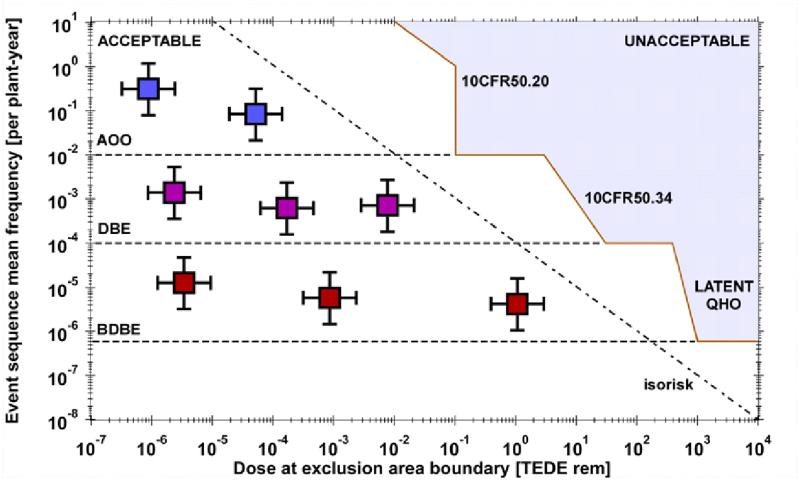
\includegraphics[width=0.90\textwidth]{farmer.jpg}
%        \caption{}
    \end{figure}
\end{frame}


\begin{frame}[plain]{}
    \centering\LARGE\textbf{\acf{npv}}
\end{frame}


\addtocounter{framenumber}{-1}
\begin{frame}{\acf{npv} is an important criterion for management}
    \begin{enumerate}[series=outerlist,topsep=0pt,itemsep=21pt,leftmargin=*,label=(\arabic*)]
        \item[]What is the relationship between 1 dollar today and 1 dollar tomorrow?
        \item[]Cost is typically the motivating factor in selecting options
        \item[]Not always the best though
        \item[]Expenditures and revenues occur over life cycle
        \item[]For \acsp{npp} much of the expenditures are up front but big
        \item[]\acs{npv} measures present value of various cash flows in different periods in the future
    \end{enumerate}
\end{frame}


\begin{frame}{Rate at which future cash flows are discounted is determined by the discount rate}
    \begin{enumerate}[series=outerlist,topsep=0pt,itemsep=17pt,leftmargin=*,label=(\arabic*)]
        \item[]$\acs{npv} > 0$ -- Wealth maximization principle
    \end{enumerate}

    \begin{equation}
        \LARGE
        \acs{npv} = \sum_{t=0}^T \; \frac{C_t}{(1 + r)^t}
    \end{equation}

    \begin{enumerate}[series=outerlist,topsep=0pt,itemsep=17pt,leftmargin=*,label=(\arabic*)]
        \item[]Maximize the current value of the investors net wealth
        \item[]Shareholders in an energy company to build a new reactor
        \item[]Current discount rates contained in \href{https://www.federalregister.gov/documents/2023/12/29/2023-28727/discount-rates-for-cost-effectiveness-analysis-of-federal-programs}{OMB Circular A-94, Appendix C}
        \item[]Must consider all relevant cash flows throughout the decision life cycle
    \end{enumerate}
\end{frame}


\begin{frame}[plain]{}
    \centering\LARGE\textbf{\href{https://uidaho.pressbooks.pub/riskassessment/chapter/decision-trees/}{Decision trees}}
\end{frame}


\addtocounter{framenumber}{-1}
\begin{frame}{}
    \begin{figure}
        \centering
        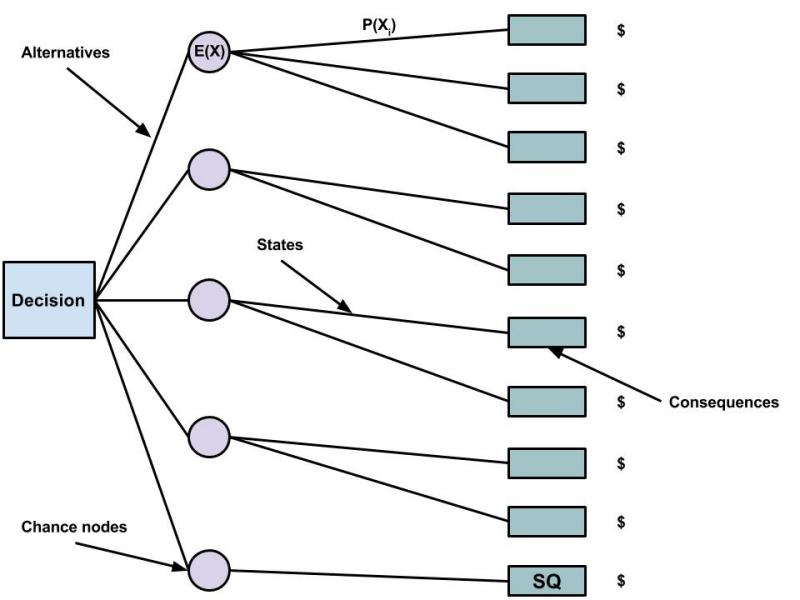
\includegraphics[width=0.80\textwidth]{decision.tree_blank.jpg}
%        \caption{}
    \end{figure}
\end{frame}


\begin{frame}{How many decisions with complete certainty have you ever made?}
    \begin{enumerate}[series=outerlist,topsep=0pt,itemsep=11pt,leftmargin=*,label=(\arabic*)]
        \item[]All decisions carry risk
        \item[]You're making decisions with imperfect knowledge  
        \item[]Does a good decision always guarantee a good outcome?
        \item[]Almost all decisions involve some level of uncertainty  
        \item[]Consequences may be large or insignificant  
        \item[]Use of a decision tree can aid in strategic thinking
        \item[]Decision making with uncertainty  
        \item[]Quantitative reasoning
        \item[]\href{https://oll.libertyfund.org/title/knight-risk-uncertainty-and-profit}{Frank Knight (1921)} famed text on the topic
    \end{enumerate}
\end{frame}


\begin{frame}[plain]{}
    \centering\LARGE\textbf{Example}
\end{frame}


\addtocounter{framenumber}{-1}
\begin{frame}{What's your decision?}
    \begin{enumerate}[series=outerlist,topsep=0pt,itemsep=21pt,leftmargin=*,label=(\arabic*)]
        \item[]Win 100 dollars calling the roll of a die even or odd
        \item[]35 dollar buy in
        \item[]I can afford to lose 35 dollars  
        \item[]I could really use 100 dollars  
        \item[]I don’t gamble
    \end{enumerate}
\end{frame}


\begin{frame}{Is 35 dollars a good buy in?}
    \begin{enumerate}[series=outerlist,topsep=0pt,itemsep=21pt,leftmargin=*,label=(\arabic*)]
        \item[]What would you negotiate?
        \item[]Decision analysis forces you to think carefully   
        \item[]Discern true nature of the decision problem by constructing a tree
        \item[]Nature of the sequential interaction of decisions and chance events
        \item[]Can only choose opportunities (pathways) not outcomes
        \item[]The outcomes are what they are 
    \end{enumerate}
\end{frame}


\begin{frame}{How do we evaluate a decision?}
    \begin{enumerate}[series=outerlist,topsep=0pt,itemsep=15pt,leftmargin=*,label=(\arabic*)]
        \item[]Decide on the decision criterion -- is it money (loss or gain)? Fatalities? Accidents? Dose? 
        \item[]Decide on a model to evaluate the criteria -- Expected value, Utility theory
        \item[]\textit{Certainty Equivalent} is when you are indifferent between a deal with at least two opportunities and a guaranteed sum of money
        \item[]Risk tolerance is on either side of that 
        \item[]Ideally you would want to know the outcome beforehand
        \item[]That is why you count cards
    \end{enumerate}
\end{frame}


\begin{frame}{Distinguish between good decisions and good outcomes}
    \begin{enumerate}[series=outerlist,topsep=0pt,itemsep=1pt,leftmargin=*,label=(\arabic*)]
        \item[]Good decisions balance good and bad outcomes in accordance with risk attitudes
            \vspace{0.10in}
        \item[]\textbf{Heterogeneity}
        \item[]Range of different outcomes  
        \item[]How bad is bad  
        \item[]How much worse is one than the other
            \vspace{0.10in}
        \item[]\textbf{Relating Probabilities to Probabilities}
        \item[]Small probabilities  
        \item[]Intuitive tendencies aren't typically correct
            \vspace{0.10in}
        \item[]\textbf{Complexity}
        \item[]Multiple outcomes and multiple probabilities
    \end{enumerate}
\end{frame}


\begin{frame}{Risk aversion is a psychological concept to settle for a lower return for a greater certainty of outcomes}
    \begin{enumerate}[series=outerlist,topsep=0pt,itemsep=15pt,leftmargin=*,label=(\arabic*)]
        \item[]People are not indifferent to uncertainty  
        \item[]Stems from uneven preferences for different outcomes
        \item[]Decreased chance of losing money
        \item[]I don't like losing 100 dollars for the chance to gain 250 dollars
        \item[]I would rather try to gain 500 dollars even if I could lose 150 dollars
        \item[]Risk averse individuals will pay risk premiums to avoid uncertainty -- fear loss and seek sureness
        \item[]Buy the half a point on a 7.5 line in football
    \end{enumerate}
\end{frame}


\begin{frame}{Risk neutral are indifferent to uncertainty}
    \begin{enumerate}[series=outerlist,topsep=0pt,itemsep=21pt,leftmargin=*,label=(\arabic*)]
        \item[]Expected value criterion is useful generally in the case where the decision maker is risk neutral
        \item[]Utility theory offers an alternative to the expected value approach
    \end{enumerate}
\end{frame}


\begin{frame}{Risk lovers hope to win big and don’t mind losing as much}
    \begin{enumerate}[series=outerlist,topsep=0pt,itemsep=21pt,leftmargin=*,label=(\arabic*)]
        \item[]Risk lover seeks to maximize the maximum gain -- maximax
        \item[]Conservative decision maker seeks to maximize the minimum gain or minimize the maximum loss -- maximin minimax
    \end{enumerate}
\end{frame}


\begin{frame}{How is this done?}
    \begin{enumerate}[series=outerlist,topsep=0pt,itemsep=21pt,leftmargin=*,label=(\arabic*)]
        \item[]Choose between a fixed sum of money $k$ and lottery in which the expected prize is $k$, you are indifferent
        \item[]Risk averse takes the fixed sum
        \item[]Risk seeker takes the lottery
        \item[]Get 100 dollars up front, or go for the lottery where the coin flip gives you 200 dollars on heads
        \item[]Expected value is not a good criterion for people who dislike risk
    \end{enumerate}
\end{frame}


\begin{frame}{A risk premium is the amount paid by a (risk averse) individual to avoid risk}
    \begin{enumerate}[series=outerlist,topsep=0pt,itemsep=21pt,leftmargin=*,label=(\arabic*)]
        \item[]Insurance premiums
        \item[]Higher fees paid by owner to reputable contractors
        \item[]Higher charges by contractor for risky work
        \item[]Lower returns from less risky investments
        \item[]Warranty?
    \end{enumerate}
\end{frame}


\begin{frame}[plain]{}
    \centering\LARGE\textbf{Bridge modifications}
\end{frame}


\addtocounter{framenumber}{-1}
\begin{frame}{}
    \begin{figure}
        \centering
        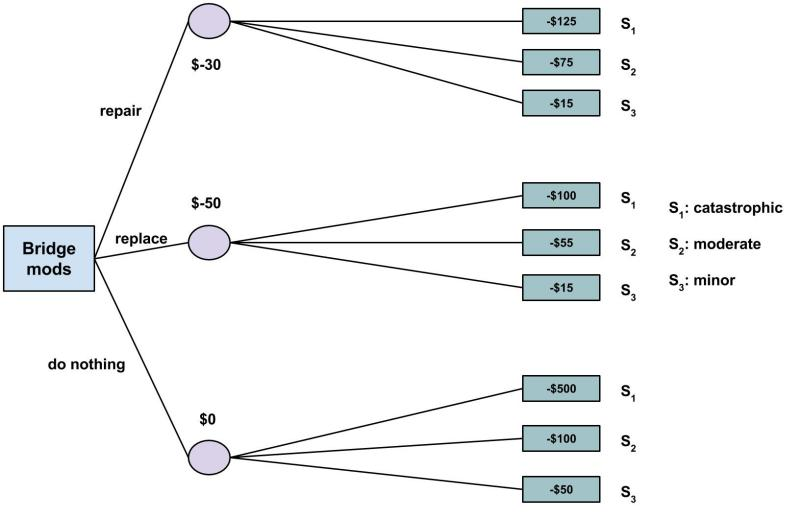
\includegraphics[width=0.80\textwidth]{bridge.mods.jpg}
%        \caption{}
    \end{figure}
\end{frame}


\begin{frame}[plain]{}
    \centering\LARGE\textbf{Upfront costs}
\end{frame}


\addtocounter{framenumber}{-1}
\begin{frame}{What is the best decision for bridge modifications?}
    \begin{enumerate}[series=outerlist,topsep=0pt,itemsep=15pt,leftmargin=*,label=(\arabic*)]
        \item[]Maximize the minimum gain
        \item[]Minimize the maximum loss
        \item[]Maximize the maximum gain
        \item[]`Do nothing' decision must be included
        \item[]30M cost to repair
        \item[]50M cost to replace
        \item[]Different losses based on the scenario and decision made
    \end{enumerate}
\end{frame}


\begin{frame}[plain]{}
    \centering\LARGE\textbf{Expected value}
\end{frame}


\addtocounter{framenumber}{-1}
\begin{frame}{}
    \begin{figure}
        \centering
        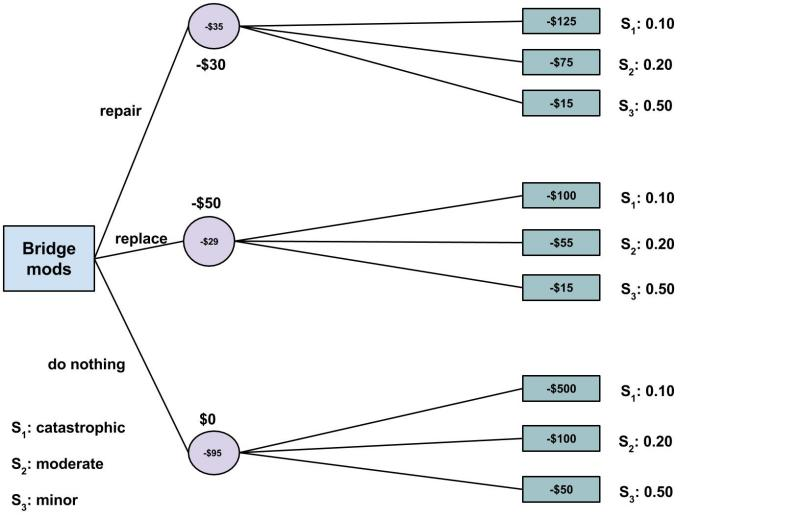
\includegraphics[width=0.80\textwidth]{bridge.mods.expected.jpg}
%        \caption{}
    \end{figure}
\end{frame}


\begin{frame}{How does the use of expected value affect decision making?}
    \begin{enumerate}[series=outerlist,topsep=0pt,itemsep=21pt,leftmargin=*,label=(\arabic*)]
        \item[]The do nothing option has the largest loss
        \item[]Going just by expected loss replacing the bridge is the best option
        \item[]Are there other factors affecting the decision besides money? 
        \item[]What other metrics could be used?
        \item[]For more complicated analysis, Bayes theory is often applied
    \end{enumerate}
\end{frame}


\begin{frame}[plain]{}
    \centering\LARGE\textbf{Hurwicz criterion}
\end{frame}


\addtocounter{framenumber}{-1}
\begin{frame}{Hurwicz criterion models a range of decision-making attitudes from conservative to optimistic}
    \begin{equation}
        \LARGE
        v(a_i,s_j) \equiv payoff
    \end{equation}

    \begin{equation}
        \LARGE
        Max(\alpha \: max \: v(a_i,s_j)+(1-\alpha) \: min \: v(a_i,s_j))
    \end{equation}

    \begin{enumerate}[series=outerlist,topsep=0pt,itemsep=11pt,leftmargin=*,label=(\arabic*)]
        \item[]$\alpha = 0$ -- minimax; risk averse
        \item[]$\alpha = 1$ -- maximax; risk seeking
        \item[]Maximize by taking the derivative and finding the optimality index and measure risk aversion
    \end{enumerate}
\end{frame}


\begin{frame}[plain]{}
    \centering\LARGE\textbf{Land use}
\end{frame}


\addtocounter{framenumber}{-1}
\begin{frame}{}
    \begin{figure}
        \centering
        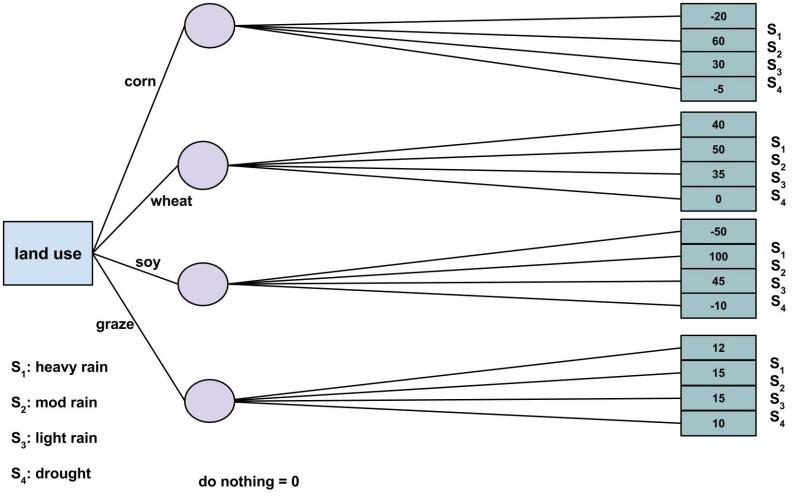
\includegraphics[width=0.80\textwidth]{land.use.template.jpg}
%        \caption{}
    \end{figure}
\end{frame}


\begin{frame}{How can we determine the best option for land use?}
    \begin{enumerate}[series=outerlist,topsep=0pt,itemsep=1pt,leftmargin=*,label=(\arabic*)]
        \item[]I did not include the do nothing option because I assumed doing nothing would result in zero for all scenarios, but there could be a lease on the land
    \end{enumerate}

    \begin{equation}
        \LARGE
        M(a_1)=60 \alpha-20(1-\alpha)
    \end{equation}

    \begin{equation}
        \LARGE
        M(a_2)=50 \alpha-0(1-\alpha)
    \end{equation}

    \begin{equation}
        \LARGE
        M(a_3)=100 \alpha-50(1-\alpha)
    \end{equation}

    \begin{equation}
        \LARGE
        M(a_4)=15 \alpha-10(1-\alpha)
    \end{equation}
\end{frame}


\begin{frame}{}
    \begin{figure}
        \centering
        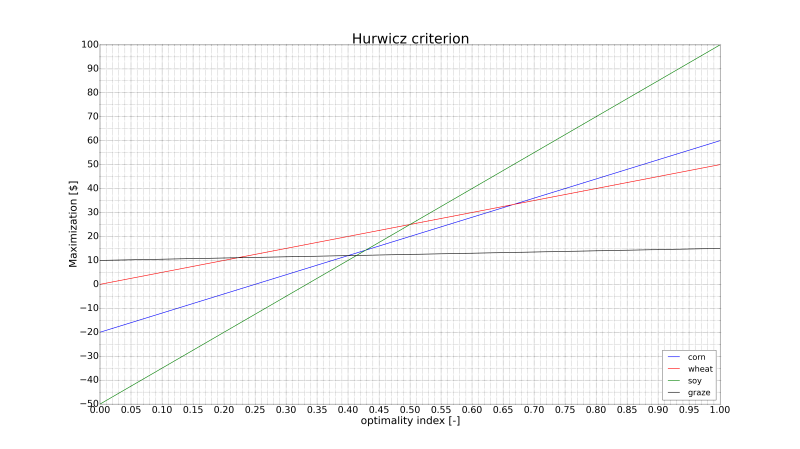
\includegraphics[width=0.95\textwidth]{land.use.hurwicz.jpg}
%        \caption{}
    \end{figure}
\end{frame}


\begin{frame}{}
    \begin{figure}
        \centering
        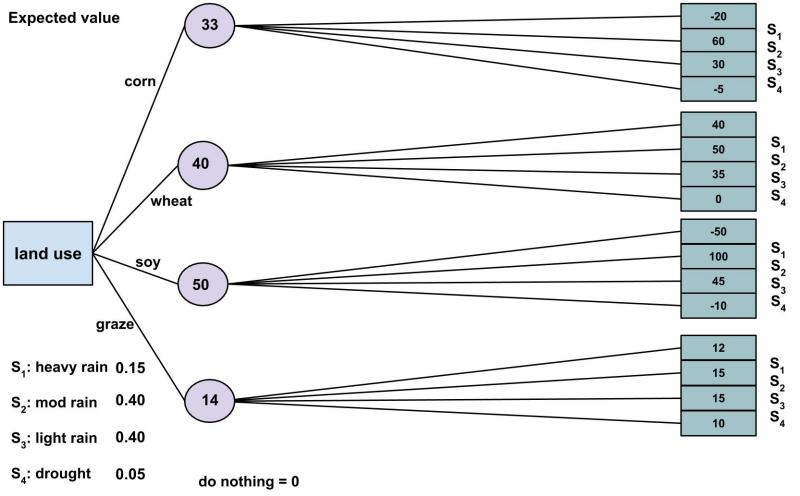
\includegraphics[width=0.90\textwidth]{land.use.expected.jpg}
%        \caption{}
    \end{figure}
\end{frame}


\begin{frame}[plain]{}
    \centering\LARGE\textbf{\href{https://uidaho.pressbooks.pub/riskassessment/chapter/utility-theory/}{Utility theory}}
\end{frame}


\addtocounter{framenumber}{-1}
\begin{frame}{Uncertain prospects are worth less in utility terms than certain ones, even when expected tangible payoffs are the same}
    \begin{enumerate}[series=outerlist,topsep=0pt,itemsep=21pt,leftmargin=*,label=(\arabic*)]
        \item[]Flip a coin    
        \item[]heads = 10M  
        \item[]tails = -9M  
        \item[]E(G) = 0.5M
        \item[]So it's a high expected payoff -- no way you play the game though
    \end{enumerate}
\end{frame}


\begin{frame}{Flip a coin and get $2^n$ for every tails in a row}
    \begin{enumerate}[series=outerlist,topsep=0pt,itemsep=11pt,leftmargin=*,label=(\arabic*)]
        \item[]How much would you pay to buy in?  
        \item[]E(1 flip) = 1 dollar    
        \item[]E(2 flip) = 2 dollars    
        \item[]E(G) = infinite  
        \item[]\href{https://policonomics.com/saint-petersburg-paradox/}{St. Petersburg paradox}
        \item[]We want to be able to measure these preferences with sound models
        \item[]Utility functions translate outcomes (\$) into pure numbers to calculate certainty equivalents consistent with a decision maker's attitude toward risk taking
        \item[]Utility of a consequence is a quantification of a person's relative preference for that consequence
    \end{enumerate}
\end{frame}


\begin{frame}{}
    \begin{figure}
        \centering
        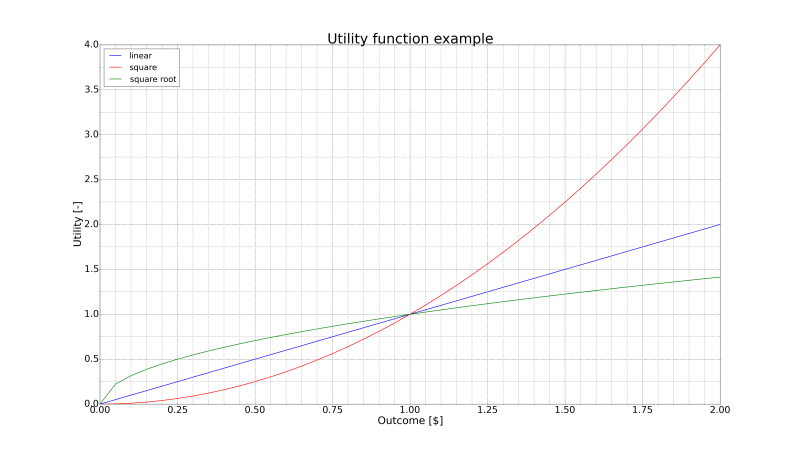
\includegraphics[width=0.95\textwidth]{utility.function.example.jpg}
%        \caption{}
    \end{figure}
\end{frame}


\begin{frame}[plain]{}
    \centering\LARGE\textbf{Expected utility}
\end{frame}


\addtocounter{framenumber}{-1}
\begin{frame}{Utility theory can give a measure of your buy in}
    \begin{enumerate}[series=outerlist,topsep=0pt,itemsep=5pt,leftmargin=*,label=(\arabic*)]
        \item[]Consider a coin flip for a 2 dollar prize
        \item[]Use expected utility instead of expected value
    \end{enumerate}

    \begin{equation}
        \LARGE
        E(u) = 0.5 \: u(0) + 0.5 \: u(2)
    \end{equation}

    \begin{equation}
        \LARGE
        u(x)=x \rightarrow E(u) = 1
    \end{equation}

    \begin{equation}
        \LARGE
        u(x)=x^2 \rightarrow E(u) = 2
    \end{equation}

    \begin{equation}
        \LARGE
        u(x)=\sqrt{x} \rightarrow E(u) = 0.71
    \end{equation}

    \begin{enumerate}[series=outerlist,topsep=0pt,itemsep=5pt,leftmargin=*,label=(\arabic*)]
        \item[]Expected utility for risk seeker is higher
    \end{enumerate}
\end{frame}


\begin{frame}{Take the inverse of the utilities to determine your buy in}
    \begin{equation}
        \LARGE
        f(E(u)) \equiv u^{-1}
    \end{equation}

    \begin{equation}
        \LARGE
        f(1)= 1
    \end{equation}

    \begin{equation}
        \LARGE
        f(2)= 1.41
    \end{equation}

    \begin{equation}
        \LARGE
        f(0.71)= 0.50
    \end{equation}

    \begin{enumerate}[series=outerlist,topsep=0pt,itemsep=5pt,leftmargin=*,label=(\arabic*)]
        \item[]Buy in is based on level of personal risk
    \end{enumerate}
\end{frame}


\begin{frame}[plain]{}
    \centering\LARGE\textbf{Data fitting}
\end{frame}


\addtocounter{framenumber}{-1}
\begin{frame}{Derive a utility function by data fit to determine risk level}
    \begin{equation}
        \LARGE
        \begin{gathered}
            \pi(x) \equiv a \: u(x) + b\\
            0 \leq \pi \leq 1 \\
            a > 0
        \end{gathered}
    \end{equation}
\end{frame}


\begin{frame}[plain]{}
    \centering\LARGE\textbf{Revisit land use}
\end{frame}


\addtocounter{framenumber}{-1}
\begin{frame}{}
    \begin{figure}
        \centering
        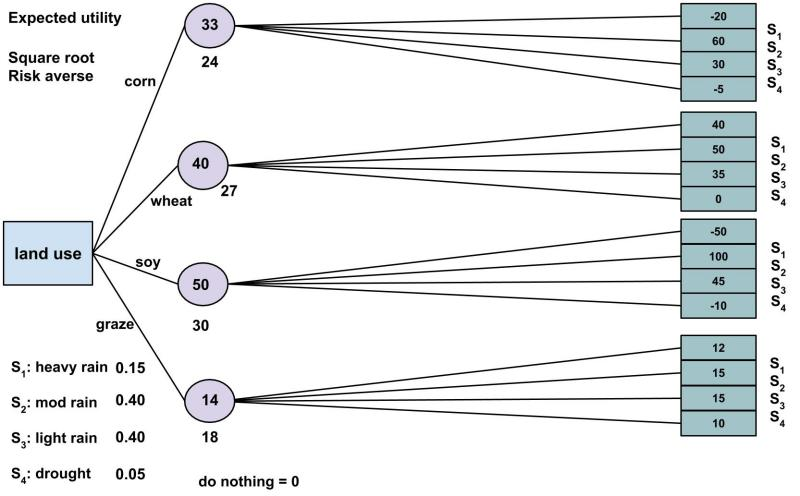
\includegraphics[width=0.80\textwidth]{decision.tree_risk.averse.jpg}
%        \caption{}
    \end{figure}
\end{frame}


\begin{frame}{}
    \begin{figure}
        \centering
        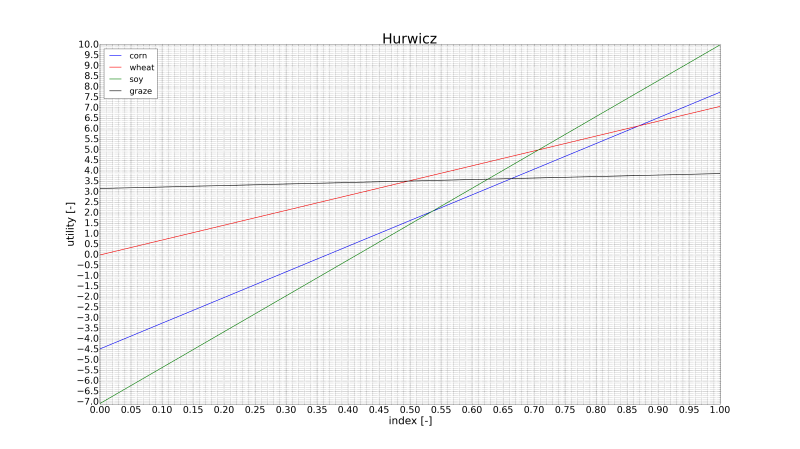
\includegraphics[width=0.95\textwidth]{hurwicz_risk.averse.jpg}
%        \caption{}
    \end{figure}
\end{frame}


\begin{frame}{}
    \begin{figure}
        \centering
        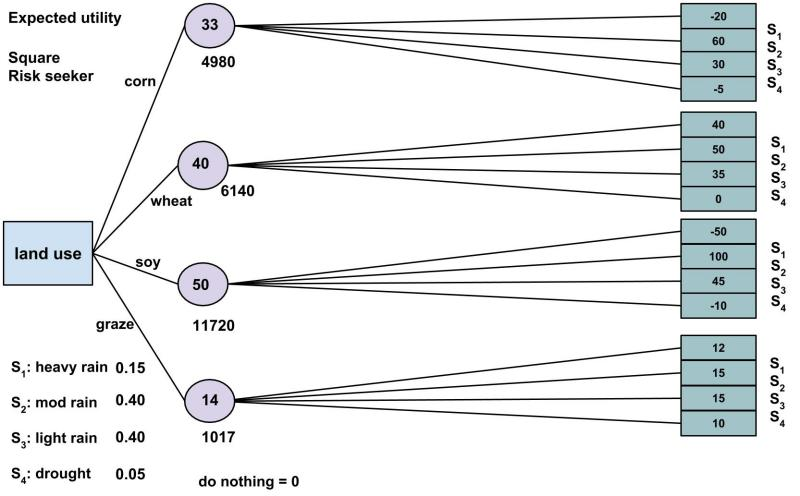
\includegraphics[width=0.80\textwidth]{decision.tree_risk.seeker.jpg}
%        \caption{}
    \end{figure}
\end{frame}


\begin{frame}{}
    \begin{figure}
        \centering
        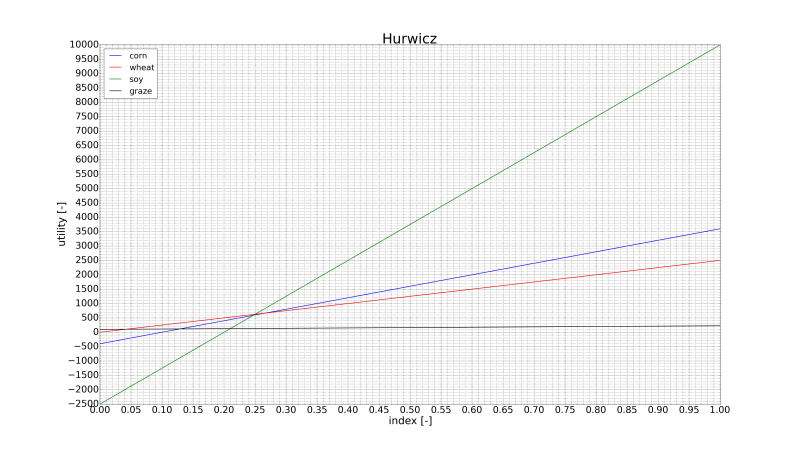
\includegraphics[width=0.95\textwidth]{hurwicz_risk.seeker.jpg}
%        \caption{}
    \end{figure}
\end{frame}


\begin{frame}{}
    \begin{figure}
        \centering
        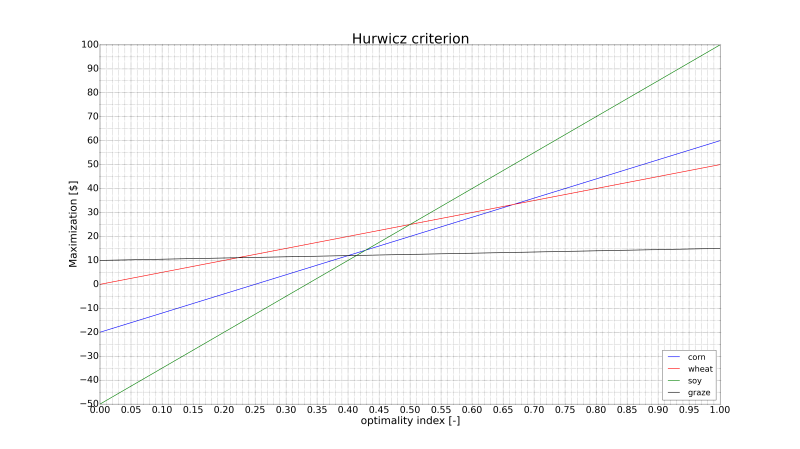
\includegraphics[width=0.80\textwidth]{land.use.hurwicz.jpg}
%        \caption{}
    \end{figure}
\end{frame}


\begin{frame}[plain]{}
    \centering\LARGE\textbf{Arrow-Pratt coefficient}
\end{frame}


\addtocounter{framenumber}{-1}
\begin{frame}{The Arrow-Pratt coefficient measures risk aversion}
    \begin{equation}
        \LARGE
        r_A(x) \equiv -\frac{u''(x)}{u'(x)}
    \end{equation}

    \begin{equation}
        \LARGE
        u(x)=x^2 \rightarrow r_A(x) = -\frac{1}{x}
    \end{equation}

    \begin{equation}
        \LARGE
        u(x)=\sqrt{x} \rightarrow r_A(x) = \frac{1}{2x}
    \end{equation}

    \begin{equation}
        \LARGE
        u(x)=1-e^{-\lambda x} \rightarrow r_A(x) = \lambda
    \end{equation}

    \begin{enumerate}[series=outerlist,topsep=0pt,itemsep=5pt,leftmargin=*,label=(\arabic*)]
        \item[]Who is the most risk averse?
    \end{enumerate}
\end{frame}


\begin{frame}{What is risk aversion like as wealth increases?}
    \begin{enumerate}[series=outerlist,topsep=0pt,itemsep=21pt,leftmargin=*,label=(\arabic*)]
        \item[]$r_A$ is positive for risk averse individuals
        \item[]Measure of curvature of preference scaling function
        \item[]Certainty equivalent is less for the more curved function
        \item[]Square root, Weibull, power law, ln(x) are common risk averse utility functions
        \item[]The higher coefficient, the more favorable odds the investor will demand in order to be willing to accept the risky bet
    \end{enumerate}
\end{frame}


\begin{frame}[plain]{}
    \centering\LARGE\textbf{Multiple attributes}
\end{frame}


\addtocounter{framenumber}{-1}
\begin{frame}{What happens when you have to measure utility for multiple attributes?}
    \begin{enumerate}[series=outerlist,topsep=0pt,itemsep=7pt,leftmargin=*,label=(\arabic*)]
        \item[]$u(x_1,x_2,x_3,...,x_n)$
        \item[]Previously we have been trying to find the utility of wealth  
        \item[]What else would we want to characterize in terms of utility?
    \end{enumerate}

    \begin{equation}
        u(x_1,x_2,x_3, \ldots ,x_n) = \sum_{i=1}^n w_i \; u_i(x_i) \: 0 \leq w_i \leq 1
    \end{equation}

    \begin{enumerate}[series=outerlist,topsep=0pt,itemsep=11pt,leftmargin=*,label=(\arabic*)]
        \item[]Assumes independence of attributes (preferences) and linearity 
        \item[]Postulate assumptions about the preference attitudes of the decision maker
        \item[]Derive functional forms of multiattribute utility function consistent with assumptions
    \end{enumerate}
\end{frame}


\begin{frame}[plain]{}
    \centering\LARGE\textbf{\acf{ahp}}
\end{frame}


\addtocounter{framenumber}{-1}
\begin{frame}{\acs{ahp} is a multiattribute decision analysis method that uses subjective judgments}
    \begin{enumerate}[series=outerlist,topsep=0pt,itemsep=13pt,leftmargin=*,label=(\arabic*)]
        \item[]\href{https://www.stat.uchicago.edu/~lekheng/meetings/mathofranking/ref/saaty1.pdf}{Decision-making with the \acs{ahp}}
        \item[]\href{https://www.sciencedirect.com/science/article/pii/0270025587904738}{The analytic hierarchy process -- what it is and how it is used}
        \item[]Alternate approach to expected utility 
        \item[]Really good for multi criteria
        \item[]Identify goal  
        \item[]Establish criteria affecting goal  
        \item[]Derive factors affecting each criteria  
        \item[]Generate alternatives
    \end{enumerate}
\end{frame}


\begin{frame}[plain]{}
    \centering\LARGE\textbf{\acs{ahp} procedure}
\end{frame}


\addtocounter{framenumber}{-1}
\begin{frame}{Make pairwise comparisons with alternatives under each criteria}
    \begin{enumerate}[series=outerlist,topsep=0pt,itemsep=1pt,leftmargin=*,label=(\arabic*)]
        \item[]Make a relative assessment between two items at a time (only 2)  
        \item[]Use objective information if possible
            \vspace{0.15in}
        \item[]1 -- elements are equally important
        \item[]3 -- one element is weakly more important  
        \item[]5 -- one element is strongly more important  
        \item[]7 -- one element is demonstrably important  
        \item[]9 -- one element is absolutely more important
        \item[]Values of 2,4,6,8 are compromises between defined categories
            \vspace{0.15in}
        \item[]Then arrange values into a matrix
    \end{enumerate}
\end{frame}


\begin{frame}{\acs{ahp} is fairly qualitative and requires kind of expert judgment}
    \begin{enumerate}[series=outerlist,topsep=0pt,itemsep=11pt,leftmargin=*,label=(\arabic*)]
        \item[]Derive consistency ratio less than 0.100
        \item[]\acs{ahp} does not require perfect consistency  
        \item[]Provides a measure of consistency
        \item[]Develop weights based on criteria and score each alternative
        \item[]Saaty suggests that hierarchies be limited to six levels and nine items per level.  
        \item[]Psychological result that people can consider 7 +/- 2 items simultaneously
        \item[]You can actually compare apples and oranges so tell people to shut up when they say that
    \end{enumerate}
\end{frame}


\begin{frame}[plain]{}
    \centering\LARGE\textbf{Yucca mountain}
\end{frame}


\addtocounter{framenumber}{-1}
\begin{frame}{}
    \begin{figure}
        \centering
        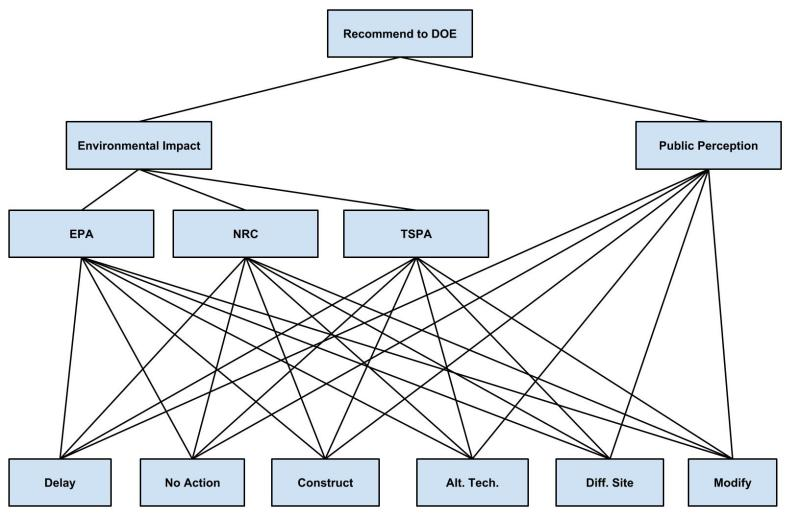
\includegraphics[width=0.80\textwidth]{ahp_first.try.jpg}
%        \caption{}
    \end{figure}
\end{frame}


\begin{frame}{This first try was overly complicated}
    \begin{enumerate}[series=outerlist,topsep=0pt,itemsep=1pt,leftmargin=*,label=(\arabic*)]
        \item[]Goal -- recommendation to \acs{doe}
        \item[]Criteria -- environmental impact and public perception
        \item[]Under environmental impact I put \acs{epa}, \acs{nrc} compliance
            \vspace{0.15in}
        \item[]\textbf{Alternatives}
        \item[]Delay -- delay to accept and construct
        \item[]No action -- do nothing
        \item[]Alt. Tech. -- alternative technologies (didn't consider \acsp{cis} at the time)
        \item[]Diff. site -- start over with a different site  
        \item[]Modify -- modify repository design (drip shield, backfill)
    \end{enumerate}
\end{frame}


\begin{frame}{Five criteria and six alternatives is a lot of pairwise comparisons}
    \begin{enumerate}[series=outerlist,topsep=0pt,itemsep=1pt,leftmargin=*,label=(\arabic*)]
        \item[]Simplify this diagram
        \item[]Could lead to high inconsistency  
            \vspace{0.10in}
        \item[]\textbf{No action 1}
        \item[]Onsite storage under institutional control for 10000 y
            \vspace{0.10in}
        \item[]\textbf{No action 2}
        \item[]Onsite storage under institutional control for 100 y
            \vspace{0.10in}
        \item[]Combine delay and modify so they can modify existing design while delaying shipments
            \vspace{0.10in}
        \item[]In hindsight, with \acsp{cis}, this would change a lot
    \end{enumerate}
\end{frame}


\begin{frame}{}
    \begin{equation}
        \LARGE
        \begin{bmatrix}
            & ENV & PP \\
            ENV & 1 & 1/3 \\
            PP & 3 & 1
        \end{bmatrix}
    \end{equation}

    \begin{equation}
        \LARGE
        \begin{bmatrix} ENV \\ PP \end{bmatrix} =
        \begin{bmatrix} 0.25 \\ 0.75 \end{bmatrix}
    \end{equation}
\end{frame}


\begin{frame}{}
    \begin{equation}
        \Large
        \begin{bmatrix}
            ENV &NA1 &NA2 &ALT &DIF &CST &D/M &EIG \\
            NA1 &1 &5 &3 &3 &2 &1/2 &0.2572 \\
            NA2 &1/5 &1 &1/3 &1/3 &1/3 &1/5 &0.0464 \\
            ALT &1/3 &3 &1 &1 &1/2 &1/3 &0.0997 \\
            DIF &1/3 &3 &1 &1 &1/3 &1/3 &0.0950 \\ 
            CST &1/2 &3 &2 &3 &1 &1/2 &0.1766 \\ 
            D/M &2 &5 &3 &3 &2 &1 &0.3251 
        \end{bmatrix} 
    \end{equation}

    \begin{enumerate}[series=outerlist,topsep=0pt,itemsep=5pt,leftmargin=*,label=(\arabic*)]
        \item[]$\acs{ci} = \frac{6.1789-6}{6-1} = 0.0358$
        \item[]$CR = 0.289$
    \end{enumerate}
\end{frame}


\begin{frame}{}
    \begin{equation}
        \LARGE
        \begin{bmatrix}
            PP &NA1 &NA2 &ALT &DIF &CST &D/M &EIG \\ 
            NA1 &1 &5 &3 &5 &1 &1/3 &0.2392 \\ 
            NA2 &1/5 &1 &1/2 &1/2 &1/2 &1/5 &0.0551 \\ 
            ALT &1/3 &2 &1 &1/2 &1/2 &1/3 &0.0825 \\ 
            DIF &1/5 &2 &2 &1 &1/3 &1/3 &0.0930 \\ 
            CST &1 &2 &2 &3 &1 &1/2 &0.1803 \\ 
            D/M &3 &5 &3 &3 &2 &1 &0.3500 
        \end{bmatrix} 
    \end{equation}

    \begin{enumerate}[series=outerlist,topsep=0pt,itemsep=5pt,leftmargin=*,label=(\arabic*)]
        \item[]$\acs{ci} = \frac{6.3716-6}{6-1} = 0.0743$
        \item[]$\acs{cr} = 0.599$
    \end{enumerate}
\end{frame}


\begin{frame}{}
    \begin{equation}
        \LARGE
        \begin{bmatrix}
            PP:ENV \; (3:1) \;\;\;\;\;\; &EIG \\ 
            NA1 &0.242 \\ 
            NA2 &0.055 \\ 
            ALT &0.090 \\ 
            DIF &0.098 \\ 
            CST &0.178 \\ 
            D/M &\textbf{0.338}
        \end{bmatrix} 
    \end{equation}
\end{frame}


\begin{frame}{}
    \begin{equation}
        \LARGE
        \begin{bmatrix}
            PP:ENV \; (1:1) \;\;\;\;\;\; &EIG \\ 
            NA1 &0.247 \\ 
            NA2 &0.052 \\ 
            ALT &0.094 \\ 
            DIF &0.097 \\ 
            CST &0.177 \\ 
            D/M &\textbf{0.332} 
        \end{bmatrix} 
    \end{equation}
\end{frame}


\begin{frame}{}
    \begin{equation}
        \LARGE
        \begin{bmatrix}
            PP:ENV \; (1:3) \;\;\;\;\;\; &EIG \\ 
            NA1 &0.251 \\ 
            NA2 &0.050 \\ 
            ALT &0.097 \\ 
            DIF &0.097 \\ 
            CST &0.177 \\ 
            D/M &\textbf{0.328}
        \end{bmatrix} 
    \end{equation}
\end{frame}


\begin{frame}{}
    \begin{figure}
        \centering
        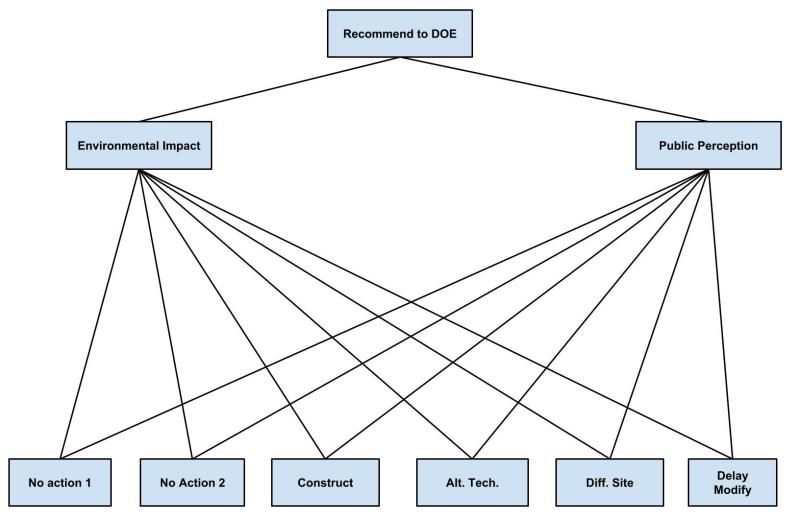
\includegraphics[width=0.80\textwidth]{ahp_final.jpg}
%        \caption{}
    \end{figure}
\end{frame}


\begin{frame}{This \acs{ahp} is more straighforward}
    \begin{enumerate}[series=outerlist,topsep=0pt,itemsep=21pt,leftmargin=*,label=(\arabic*)]
        \item[]\acs{nrc} criterion removed because it kicks in after construction
        \item[]\acs{epa} criterion folded into Environmental Impact
        \item[]No action split into 1 and 2 based on analysis of environmental impact statement
        \item[]Delay and Modify can be combined
    \end{enumerate}
\end{frame}


\begin{frame}[plain]{}
    \centering\LARGE\textbf{Buying a car}
\end{frame}


\addtocounter{framenumber}{-1}
\begin{frame}{}
    \begin{figure}
        \centering
        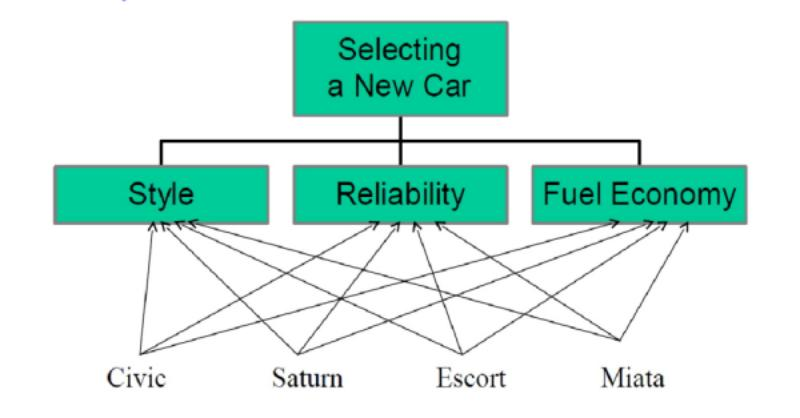
\includegraphics[width=0.80\textwidth]{ahp.car.jpg}
%        \caption{}
    \end{figure}
\end{frame}


\begin{frame}[plain]{}
    \centering\LARGE\textbf{Anything missing?}
\end{frame}


\addtocounter{framenumber}{-1}
\begin{frame}{Derive \acs{ahp} pairwise matrix}
    \begin{equation}
        \LARGE
        \begin{bmatrix}
               &A1 &A2 &A3 \\ 
            A1 &a_{11} &a_{12} &a_{13} \\ 
            A2 &a_{21} &a_{22} &a_{23} \\ 
            A3 &a_{31} &a_{32} &a_{33}
        \end{bmatrix} 
    \end{equation}

    \begin{enumerate}[series=outerlist,topsep=0pt,itemsep=5pt,leftmargin=*,label=(\arabic*)]
        \item[]$a_{ii}=1$
        \item[]$a_{ij}=a^{-1}_{ji}$
    \end{enumerate}
\end{frame}


\begin{frame}{Make pairwise comparisons}
    \begin{figure}
        \centering
        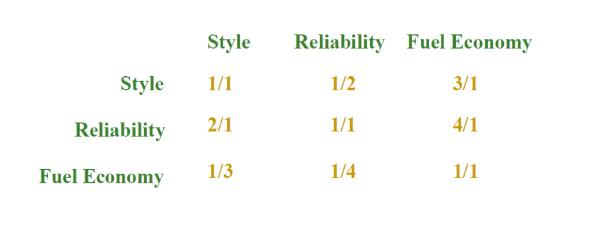
\includegraphics[width=0.80\textwidth]{ahp_car.criteria.jpg}
%        \caption{}
    \end{figure}
\end{frame}


\begin{frame}{Calculate weights}
    \begin{equation}
        \LARGE
        \begin{bmatrix} STY \\ REL \\ FE \end{bmatrix} = \begin{bmatrix} 0.3196 \\ 0.5584 \\ 0.1220 \end{bmatrix}
    \end{equation}
\end{frame}


\begin{frame}{Let's check the consistency of the criteria}
    \begin{enumerate}[series=outerlist,topsep=0pt,itemsep=1pt,leftmargin=*,label=(\arabic*)]
        \item[]$\acs{ci} = \frac{3.0183-3}{3-1} = 0.0091$
        \item[]$\acs{cr} = 0.158$
            \vspace{0.25in}
        \item[]Divide below for n criteria
    \end{enumerate}

    \begin{figure}
        \centering
        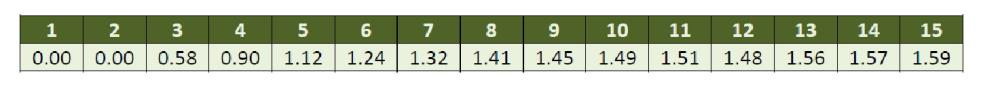
\includegraphics[width=0.85\textwidth]{cr.table.jpg}
%        \caption{}
    \end{figure}
\end{frame}


\begin{frame}{To rank the criteria, determine the eigenvector}
    \begin{equation}
        \LARGE
        \underline{\underline{A}} \: \underline{x} = \lambda \underline{x}
    \end{equation}

    \begin{equation}
        \LARGE
        |A -\lambda I| = 0
    \end{equation}
\end{frame}


\begin{frame}{Find \textit{normalized} eigenvector for greatest eigenvalue (real valued)}
    \begin{enumerate}[series=outerlist,topsep=0pt,itemsep=21pt,leftmargin=*,label=(\arabic*)]
        \item[]Eigenvalue should be slightly $> n$
        \item[]python of course (one line of code) but plenty of online tools 
        \item[]There are n eigenvalues/vectors for an n x n matrix
        \item[]Because the judgment cannot be truly consistent, we assume it exhibits a small perturbation and can satisfy the eigenvalue equation
        \item[]Measure consistency to prove this
        \item[]Deviation should only be small
    \end{enumerate}
\end{frame}


\begin{frame}{}
    \begin{figure}
        \centering
        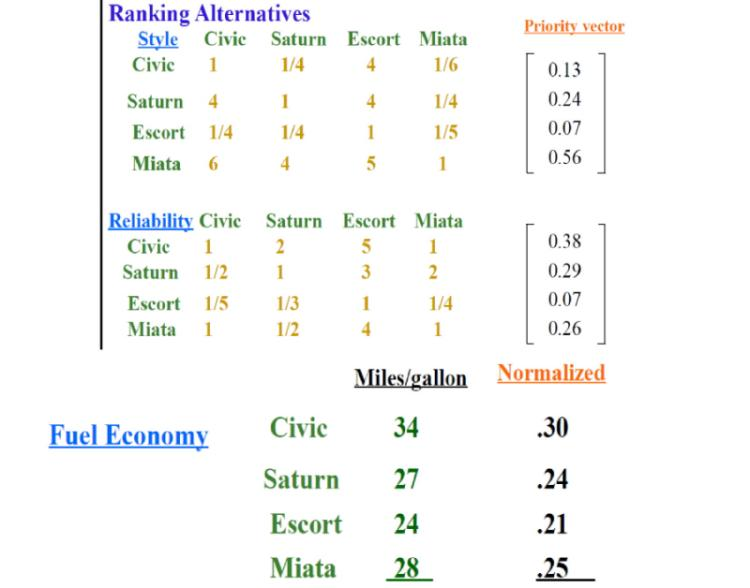
\includegraphics[width=0.75\textwidth]{ahp_car.rank.jpg}
%        \caption{}
    \end{figure}
\end{frame}


\begin{frame}{}
    \begin{figure}
        \centering
        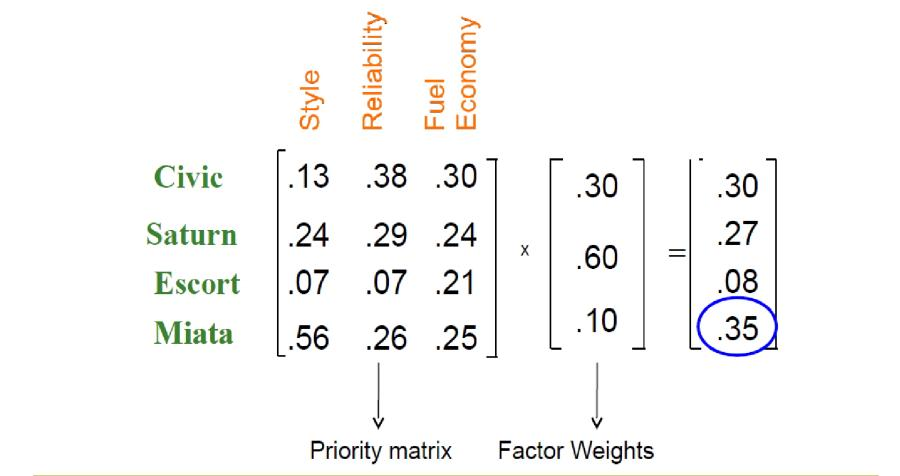
\includegraphics[width=0.80\textwidth]{ahp_car.priority.jpg}
%        \caption{}
    \end{figure}
\end{frame}


\begin{frame}{Then for some reason they brough in cost at the end}
    \begin{figure}
        \centering
        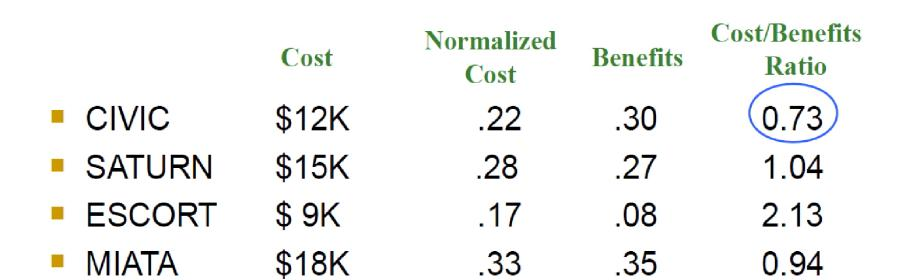
\includegraphics[width=0.80\textwidth]{ahp_cost.jpg}
%        \caption{}
    \end{figure}

    \begin{enumerate}[series=outerlist,topsep=0pt,itemsep=21pt,leftmargin=*,label=(\arabic*)]
        \item[]Do not agree
        \item[]No pairwise comparison of cost with other criteria
    \end{enumerate}
\end{frame}


\begin{frame}[plain]{}
    \centering\LARGE\textbf{Apartment}
\end{frame}


\addtocounter{framenumber}{-1}
\begin{frame}{Variable list}
    \begin{columns}[t]

        \begin{column}{0.50\textwidth}
            \begin{enumerate}[series=outerlist,topsep=0pt,itemsep=3pt,leftmargin=*,label=(\arabic*)]
                \item[]WC -- walk to campus - 30 min
                \item[]RC -- ride to campus - 15 min
                \item[]WG -- walk to groceries - 15 min
                \item[]RG -- ride to groceries
                \item[]WIC -- walk in closet
                \item[]2U -- 2 utilities included
                \item[]NOU -- no utilities included
                \item[]2+U -- more than 2 utilities included
                \item[]ES -- extra storage
            \end{enumerate}
        \end{column}

        \begin{column}{0.50\textwidth}
            \begin{enumerate}[series=outerlist,topsep=0pt,itemsep=3pt,leftmargin=*,label=(\arabic*)]
                \item[]R1 -- 600 - 699
                \item[]R2 -- 700 - 799
                \item[]R3 -- 800 - 899
                \item[]S1 -- 250 - 349 sq ft
                \item[]S2 -- 350 - 449 sq ft
                \item[]S3 -- 450+ sq ft
                \item[]MISC -- quality, laundry, etc.
            \end{enumerate}
        \end{column}

    \end{columns}
\end{frame}


\begin{frame}{}
    \begin{figure}
        \centering
        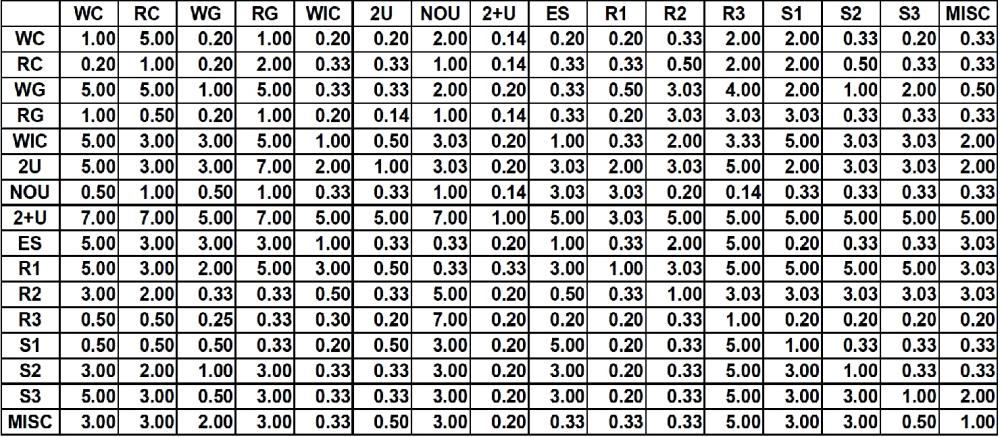
\includegraphics[width=0.90\textwidth]{ahp_apartment.jpg}
%        \caption{}
    \end{figure}

    \begin{enumerate}[series=outerlist,topsep=0pt,itemsep=1pt,leftmargin=*,label=(\arabic*)]
        \item[]$n = 16$
        \item[]$\acs{ci} = 0.327148$
        \item[]$\lambda_m = 20.907222$
        \item[]$\acs{cr} = 0.2046$
    \end{enumerate}
\end{frame}


\begin{frame}{}
    \begin{equation}
        \underline{\lambda} = 
        \begin{bmatrix}
            0.084582 \\
            0.075686 \\
            0.190081 \\
            0.073716 \\
            0.271129 \\
            0.335294 \\
            0.123018 \\
            0.657367 \\
            0.179078 \\
            0.355715 \\
            0.195451 \\
            0.080527 \\
            0.127037 \\
            0.155506 \\
            0.197643 \\
            0.172291
        \end{bmatrix}
    \end{equation}
\end{frame}


\begin{frame}{\href{https://maps.app.goo.gl/Au6WsY4nKWzXmruq9}{Normalized eigenvector}}
    \begin{columns}[t]

        \begin{column}{0.50\textwidth}
            \begin{enumerate}[series=outerlist,topsep=0pt,itemsep=3pt,leftmargin=*,label=(\arabic*)]
                \item[]WC -- 0.025834   
                \item[]RC -- 0.023116
                \item[]WG -- 0.058055
                \item[]RG -- 0.022515
                \item[]WIC -- 0.082810
                \item[]2U -- 0.102407
                \item[]NOU -- 0.037573
                \item[]2+U -- 0.200777
                \item[]ES -- 0.054695
            \end{enumerate}
        \end{column}

        \begin{column}{0.50\textwidth}
            \begin{enumerate}[series=outerlist,topsep=0pt,itemsep=3pt,leftmargin=*,label=(\arabic*)]
                \item[]R1 -- 0.108644
                \item[]R2 -- 0.059696
                \item[]R3 -- 0.024595
                \item[]S1 -- 0.038800
                \item[]S2 -- 0.047496
                \item[]S3 -- 0.060365 
                \item[]MISC -- 0.052622
            \end{enumerate}
        \end{column}

    \end{columns}
\end{frame}


\begin{frame}[plain]{}
    \centering\LARGE\textbf{Fuzzy logic}
\end{frame}


\addtocounter{framenumber}{-1}
\begin{frame}{Fuzzy (set theory) logic captures the truth in `usually'}
    \begin{enumerate}[series=outerlist,topsep=0pt,itemsep=15pt,leftmargin=*,label=(\arabic*)]
        \item[]Boolean logic states that a concept is either true or false -- $1 \equiv true$, $0 \equiv false$
        \item[]Fuzzy logic posits that a concept possesses a degree of truth varying between 0 and 1 
        \item[]Applicable to vague, or subjectively judged, concepts
        \item[]The coffee is hot
        \item[]It could be scorching or mildly hot
        \item[]Fuzzy logic represents uncertain information
        \item[]Focuses on formal principles of approximate reasoning or imprecise modes of reasoning
        \item[]Captures uncertainty inherent in subjective judgements
    \end{enumerate}
\end{frame}


\begin{frame}[plain]{}
    \centering\LARGE\textbf{Procedure}
\end{frame}


\addtocounter{framenumber}{-1}
\begin{frame}{Define linguistic variables}
    \begin{enumerate}[series=outerlist,topsep=0pt,itemsep=15pt,leftmargin=*,label=(\arabic*)]
        \item[]Very High, High, Moderate, Low, Very Low
        \item[]Or the \acs{ahp} scale
        \item[]Map the linguistic variables to membership functions
        \item[]Used when there are a lot of people making judgements 
        \item[]Fuzzy rules (if-then) are derived if needed
        \item[]If X is Low and Y is High, then the result is Moderate, etc., for all the combinations
    \end{enumerate}
\end{frame}


\begin{frame}{}
    \begin{equation}
        \LARGE
         \tilde{\chi} \equiv (l,m,n,s)
    \end{equation}

    \begin{equation}
        \LARGE
        \mu(\chi)=
    \begin{cases}
        0 & \; \chi < l \\
        \frac{\chi-l}{m-l} & \; l \leq \chi \leq m \\
        1 & \; m \leq \chi \leq n \\
        \frac{s-\chi}{s-n} & \; n \leq \chi \leq s \\
        0 & \; \chi > s
    \end{cases}
    \end{equation}
\end{frame}


\begin{frame}{}
    \begin{figure}
        \centering
        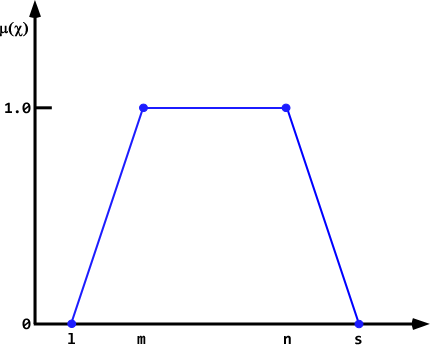
\includegraphics[width=0.70\textwidth]{fuzzy-ahp-membership.png}
%        \caption{}
    \end{figure}
\end{frame}


\begin{frame}{Mapping the five point scale}
    \begin{enumerate}[series=outerlist,topsep=0pt,itemsep=15pt,leftmargin=*,label=(\arabic*)]
        \item[]Very high -- (4,4.5,5,5) (7,8,9,10)
        \item[]High -- (3,3.5,4.5,5)    (5,6,7,8)
        \item[]Moderate -- (2,2.5,3.5,4)(3,4,5,6) 
        \item[]Low -- (1,1.5,2.5,3)     (1,2,3,4) 
        \item[]Very Low -- (1,1,1.5,2)  (0,1,2,3)
    \end{enumerate}
\end{frame}


\begin{frame}{More math}
    \begin{enumerate}[series=outerlist,topsep=0pt,itemsep=21pt,leftmargin=*,label=(\arabic*)]
        \item[]Typically, take the geometric mean of the membership functions to aggregate them into a single membership function
        \item[]Take the centroid of the function to obtain the final `crisp number'
        \item[]The end result could just be a ranking of criteria, measure of risk, etc.
        \item[]The fuzzy math takes into account the uncertainties in the judgements
    \end{enumerate}
\end{frame}


\begin{frame}[plain]{}
    \centering\LARGE\textbf{\href{https://www.sciencedirect.com/science/article/pii/S0149197021004352}{Fuzzy \acs{ahp}}}
\end{frame}


\begin{frame}[plain]{}
    \centering\LARGE\textbf{Risk perception and communication}
\end{frame}


\addtocounter{framenumber}{-2}
\begin{frame}{Effective communication of risk involves understanding risk perception}
    \begin{enumerate}[series=outerlist,topsep=0pt,itemsep=21pt,leftmargin=*,label=(\arabic*)]
        \item[]
            \begin{quote}
                What we had done to these people was just outrageous. We had frightened them so bad, they thought they were going to die. \\
                --\acs{nrc} official describing government communication during Three Mile Island
            \end{quote}
        \item[]Public perceives and responds to risky situations based on emotion in addition to facts (which is fine)
        \item[]Sabine Roeser is the expert in the role of emotion and risk  
        \item[]Emotion is a rational process
    \end{enumerate}
\end{frame}


\begin{frame}{Nuclear risk is the most difficult risks and nuclear experts have to be the most socially literate}
    \begin{enumerate}[series=outerlist,topsep=0pt,itemsep=21pt,leftmargin=*,label=(\arabic*)]
        \item[]
            \begin{quote}
                Emotion can play a bigger role in the way people perceive risks, than reason and rational thinking.\\
                --Paul Slovic, Affect heuristic
            \end{quote}
        \item[]Emerging technologies exhibit a different paradigm and require different approaches
        \item[]I don't like use of `the public' because it frames a us v them mentality
        \item[]Aren't we all the public
    \end{enumerate}
\end{frame}


\begin{frame}{Nuclear engineering is unique because of `historical inertia'}
    \begin{enumerate}[series=outerlist,topsep=0pt,itemsep=21pt,leftmargin=*,label=(\arabic*)]
        \item[]
            \begin{quote}
                The unleashed power of the atom has changed everything except our modes of thinking, and thus we drift toward unparalleled catastrophes. We shall require a substantially new manner of thinking if humanity is to survive.\\
                --Einstein, August 1964 New York Times Magazine
            \end{quote}
        \item[]
            \begin{quote}
                Consensus is tricky. Disagreement has always been a part of science. However, I find now that in the era of `armchair' science - many people just don't understand the scientific process, the peer-review process, etc. They see thing more like a legal system and reasonable doubt. If there is reasonable doubt or slight uncertainty, they think the basic scientific premise is flawed. Science doesn't work that way.\\
                --Marshall Shepherd, 2013 President American Meteorological Society
            \end{quote}
        \item[]Complaining about it isn't fixing it
    \end{enumerate}
\end{frame}


\begin{frame}{Nuclear and radiological risks feel more frightening to the public}
    \begin{enumerate}[series=outerlist,topsep=0pt,itemsep=21pt,leftmargin=*,label=(\arabic*)]
        \item[]If they don't feel `safe' then they aren't safe so it doesn't matter what the facts are
        \item[]\href{https://slideplayer.com/slide/4189923/}{These characteristics must be acknowledged in order to effectively manage public behavior} (slide 6)
        \item[]Ridiculously arrogant and could not be more wrong
        \item[]\textit{Meet people where they are}
        \item[]What is important to others may not be what you think it is
    \end{enumerate}
\end{frame}


\begin{frame}{What affects risk perception?}
    \begin{enumerate}[series=outerlist,topsep=0pt,itemsep=1pt,leftmargin=*,label=(\arabic*)]
        \item[]Media attention
        \item[]Familiarity
        \item[]Scientific certainty    
        \item[]History or historical inertia
        \item[]Reversibility
        \item[]Trust
        \item[]Benefits  
        \item[]Fairness of risk distribution
        \item[]Nature of risk
        \item[]Catastrophic potential v chronic (low probability/high consequence -- high probability/low consequence) 
        \item[]Uncertainty
        \item[]Fear
        \item[]Influence on children and future generations  
    \end{enumerate}
\end{frame}


\begin{frame}{What else affects risk perception?}
    \begin{enumerate}[series=outerlist,topsep=0pt,itemsep=21pt,leftmargin=*,label=(\arabic*)]
        \item[]Voluntary v involuntary risk
        \item[]Driving a car v flying even though flying is lower risk and the airlines are organized crime syndicates
        \item[]The risk manager must \ldots deal not only with risk perceived through science, but also with virtual risk -- risks where the science is inconclusive and people are thus liberated to argue from, and act upon, preestablished beliefs, convictions, prejudices and superstitions. \href{https://www.proquest.com/docview/227006505/fulltextPDF/2985AF92A8EE48CFPQ/1?accountid=14551&sourcetype=Magazines}{(Risk Management Magazine)}
    \end{enumerate}
\end{frame}


\begin{frame}{Establishing trust is the primary factor in effective communication}
    \begin{enumerate}[series=outerlist,topsep=0pt,itemsep=17pt,leftmargin=*,label=(\arabic*)]
        \item[]Admit when mistakes have been made  
        \item[]Avoid secrets
        \item[]Dialogue and respect for audience feelings must be sincere
        \item[]Veracity = sincere AND honest
        \item[]\textit{Oh, I'm just being honest.} No, you're being a bag.
        \item[]Do not tell people how they should feel  
        \item[]That makes me feel angry!
        \item[]Do not over reassure either though
    \end{enumerate}
\end{frame}


\begin{frame}{\acs{cdc} recommends preparing for the following risk questions when dealing with the public}
    \begin{enumerate}[series=outerlist,topsep=0pt,itemsep=15pt,leftmargin=*,label=(\arabic*)]
        \item[]Why did this happen?
        \item[]Why wasn't this prevented?
        \item[]What else can go wrong?
        \item[]When were you notified about this?
        \item[]What does this information mean?
        \item[]How are ill going to get help?
        \item[]What can we expect?
        \item[]What bad things aren't you telling us?
    \end{enumerate}
\end{frame}


\begin{frame}{}
    \begin{figure}
        \centering
        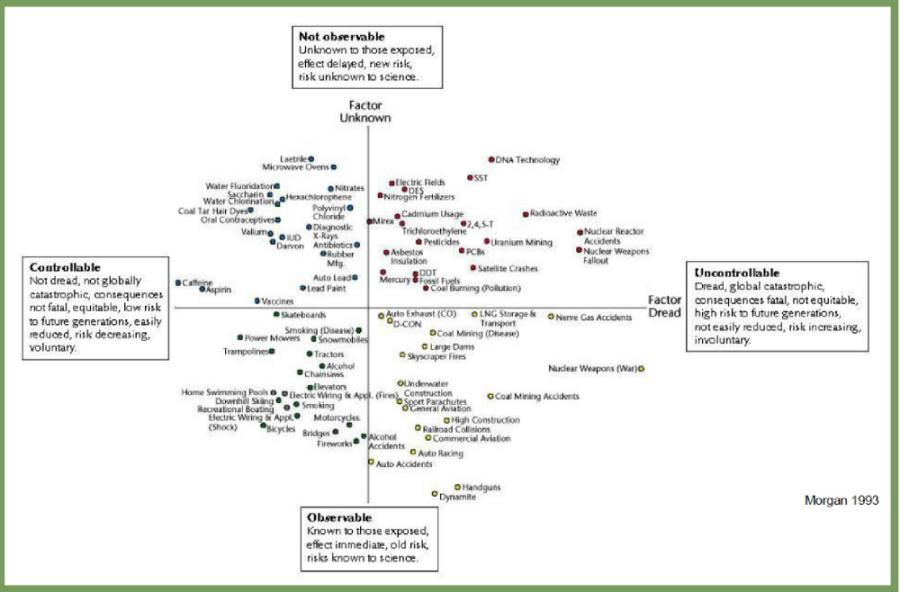
\includegraphics[width=0.80\textwidth]{risk.chart.jpg}
%        \caption{}
    \end{figure}
\end{frame}


\begin{frame}{No single level of risk that society finds acceptable}
    \begin{enumerate}[series=outerlist,topsep=0pt,itemsep=15pt,leftmargin=*,label=(\arabic*)]
        \item[]This is why there are regulations, but people may not accept that either
        \item[]Risks that society is prepared to accept or tolerate will vary from situation to situation
        \item[]Localities v Las Vegas for Yucca Mountain  
        \item[]Just about every waste repository case was a failure in communication -- Japan, South Korea 
        \item[]Community needs to be involved -- Finland, Sweden
        \item[]Long time scales, irreversibility, complexity hard to communicate
    \end{enumerate}
\end{frame}


\begin{frame}{Learning how to talk to people isn't so easy}
    \begin{enumerate}[series=outerlist,topsep=0pt,itemsep=15pt,leftmargin=*,label=(\arabic*)]
        \item[]Talk local and personal
        \item[]Talk about concrete facts and issues, not abstract
        \item[]Talk about what is happening now, not later  
        \item[]Emphasize trade offs with risks and benefits
        \item[]Talk about increasing consequences if delaying and doing nothing -- If that's actually true
        \item[]Talk about manageable solutions
        \item[]Meet people where they are
        \item[]Social scientists are critically important -- \acs{doe} \acs{cis} funding was social science-led. Shocker.
    \end{enumerate}
\end{frame}


\begin{frame}{\acs{epa} has seven cardinal rules of risk communication}
    \begin{enumerate}[series=outerlist,topsep=0pt,itemsep=15pt,leftmargin=*,label=(\arabic*)]
        \item[]Accept and involve the public as a legitimate partner
        \item[]Listen to the audience -- Meet people where they are 
        \item[]Be honest, frank, and open -- Veracity 
        \item[]Coordinate and collaborate with other credible sources
        \item[]Meet the needs of the media
        \item[]Speak clearly and with compassion -- Not everyone can do this
        \item[]Plan carefully and evaluate performance
    \end{enumerate}
\end{frame}


\begin{frame}[plain]{}
    \begin{figure}
        \centering
        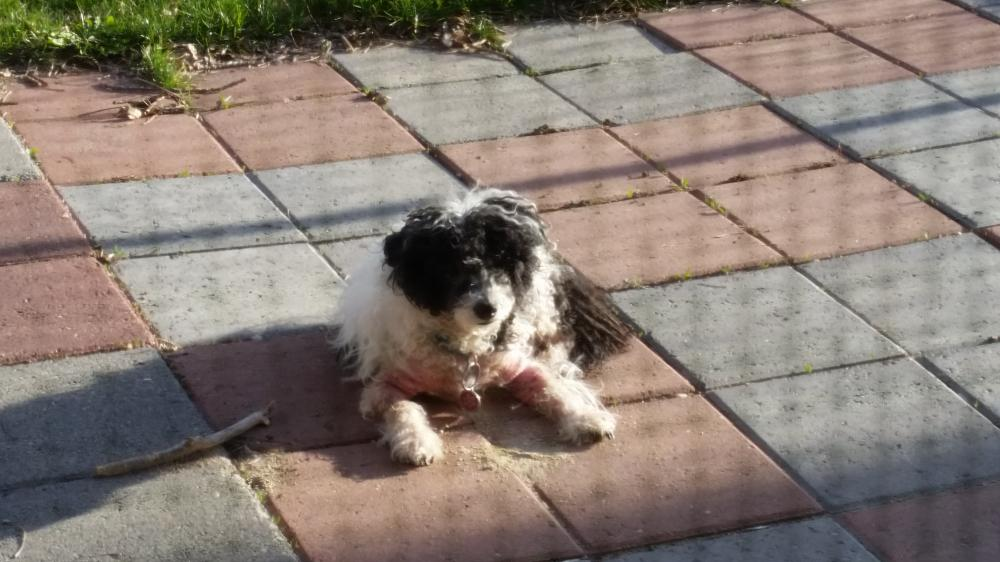
\includegraphics[width=0.85\textwidth]{final.jpg}
%        \caption{}
    \end{figure}
\end{frame}


%%%%%%%
%\begin{frame}{}
%    \begin{columns}
%
%        \begin{column}{0.50\textwidth}
%            \begin{enumerate}[series=outerlist,topsep=0pt,itemsep=21pt,leftmargin=*,label=(\arabic*)]
%                \item[]
%                \item[]
%            \end{enumerate}
%        \end{column}
%
%        \begin{column}{0.50\textwidth}
%            \begin{enumerate}[series=outerlist,topsep=0pt,itemsep=21pt,leftmargin=*,label=(\arabic*)]
%                \item[]
%                \item[]
%            \end{enumerate}
%        \end{column}
%
%    \end{columns}
%\end{frame}

%    \begin{figure}
%        \centering
%        \includegraphics[width=0.75\textwidth]{wsc.png}
%        \caption{\acs{wsc}}
%    \end{figure}


%\begin{frame}{References}
%    \bibliographystyle{nsf}
%    \footnotesize
%    \bibliography{references}
%\end{frame}
%%%%%%%


\end{document}
